\newpage 
\section{2 lepton ATLAS data analysis}

The 3 lepton + $e_T^{miss}$ dataset has less events, and thus allows for less training of the neural networks. 
Thus, the 2 lepton + $e_T^{miss}$ dataset was tried instead. The event selection was done choosing atleast 
2 leptons, meaning that the RMM signatures of some of the events will look similar to the RMM signatures of 
the 3 lepton + $e_T^{miss}$ dataset. A consequence of this is that the signal samples for the 3 lepton case 
would be a good start point for testing. The signal region for the regular autoencoder models were created by 
calculating the median $m_{err}$ of the reconstruction error. Then, 3 cuts were made, starting at 
$m_{err} + im_{err}/5$ for $i = 1,2,3$. As the shape of the background reconstruction error has a hill like 
shape, the median is a good place to start to remove alot of the background. This is however just a guess 
for an optimal signal region, as the true signal is unknown, and the method has to be as unbiased as possible. 
Below are some of the results from training on the 2 lepton case, using the same two SUSY signals as test cases. 


\begin{figure}[H]
    \centering
    \begin{subfigure}{.45\textwidth}
        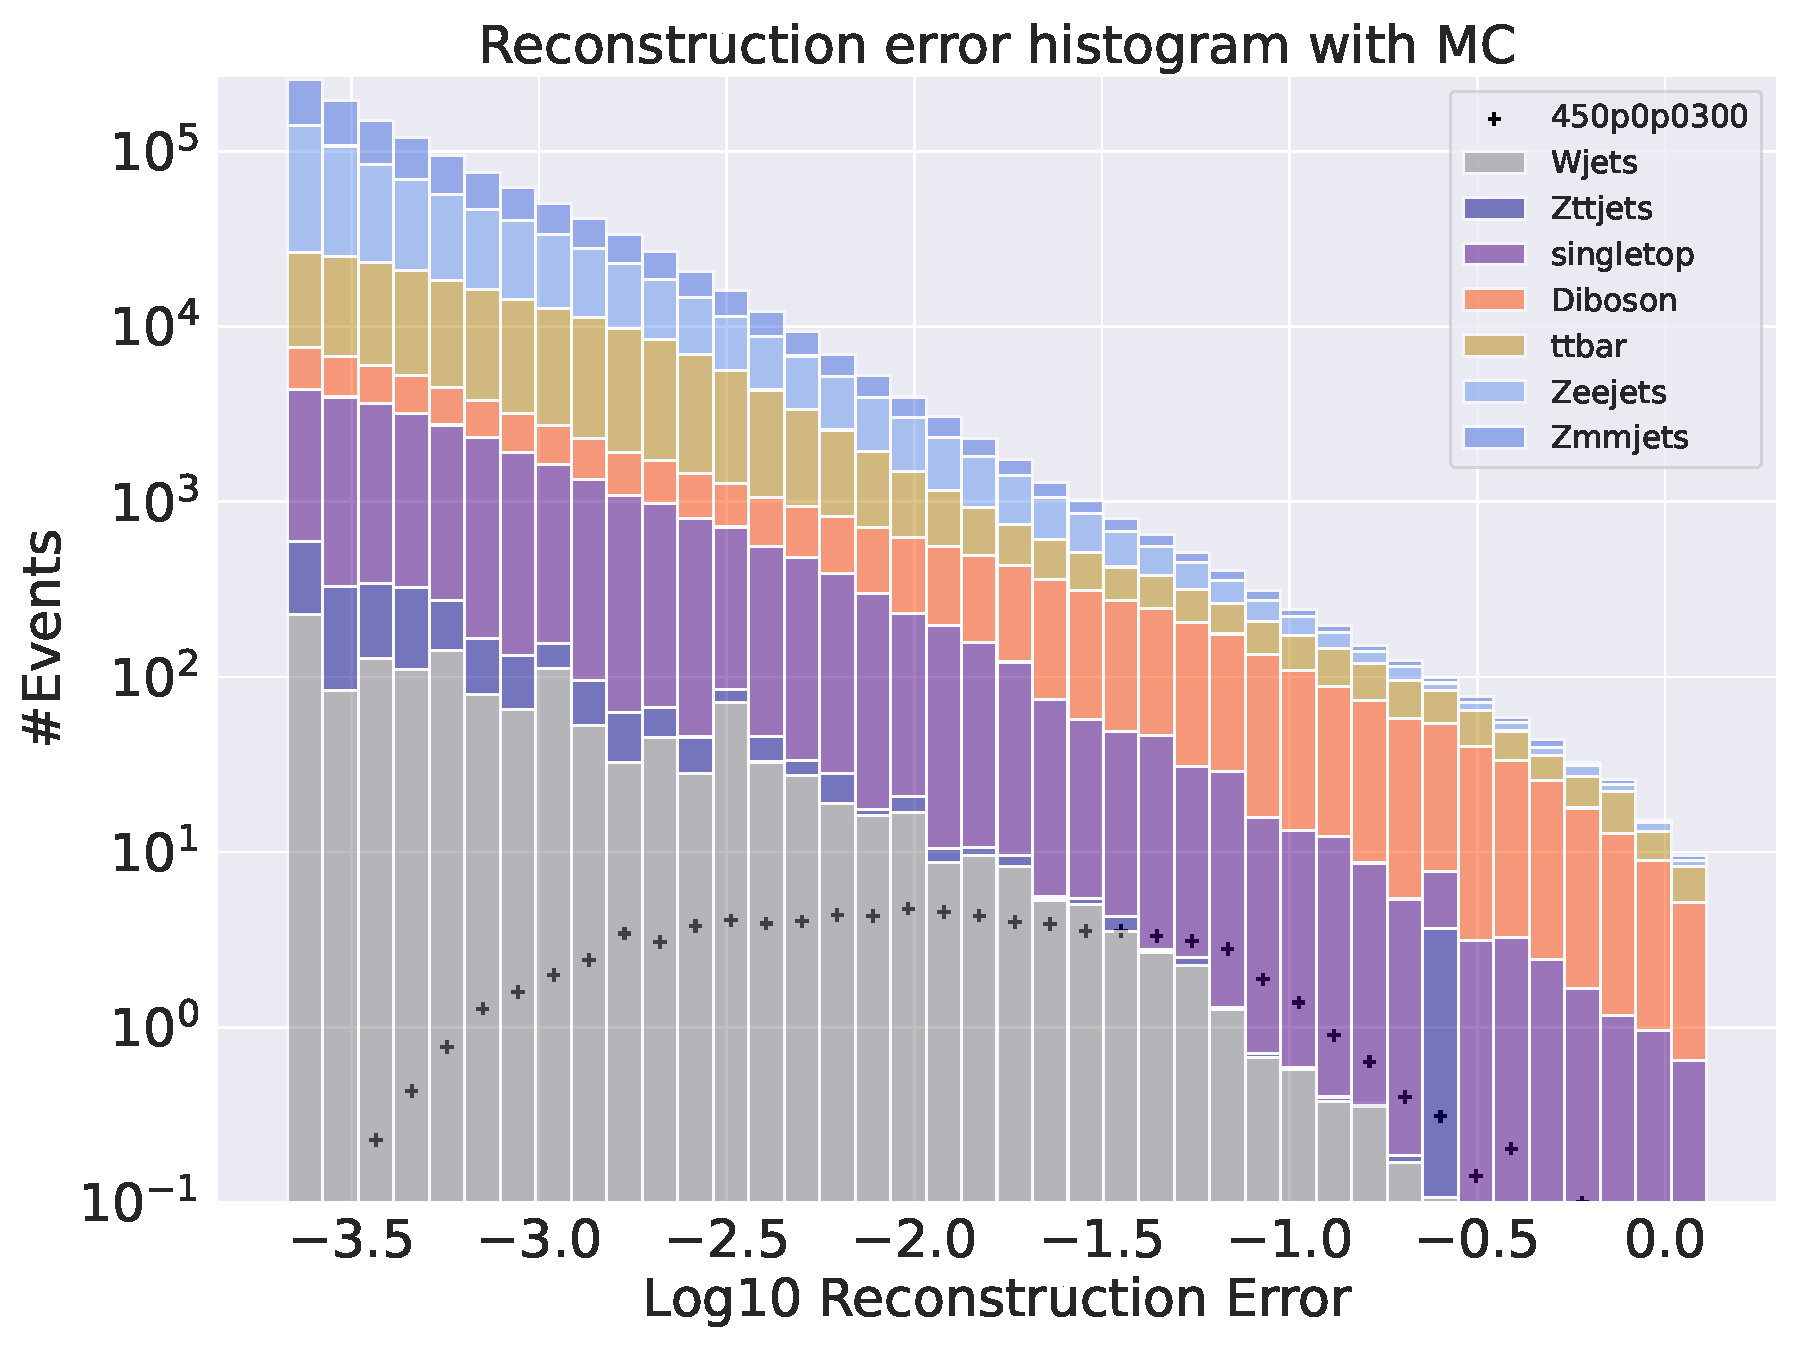
\includegraphics[width=\textwidth]{Figures/AE_testing/big/2lep/b_data_recon_big_rm3_feats_sig_450p0p0300_.pdf}
        \caption{ }
        \label{fig:AE_2lep_big_450}
    \end{subfigure}
    \hfill
    \begin{subfigure}{.45\textwidth}
        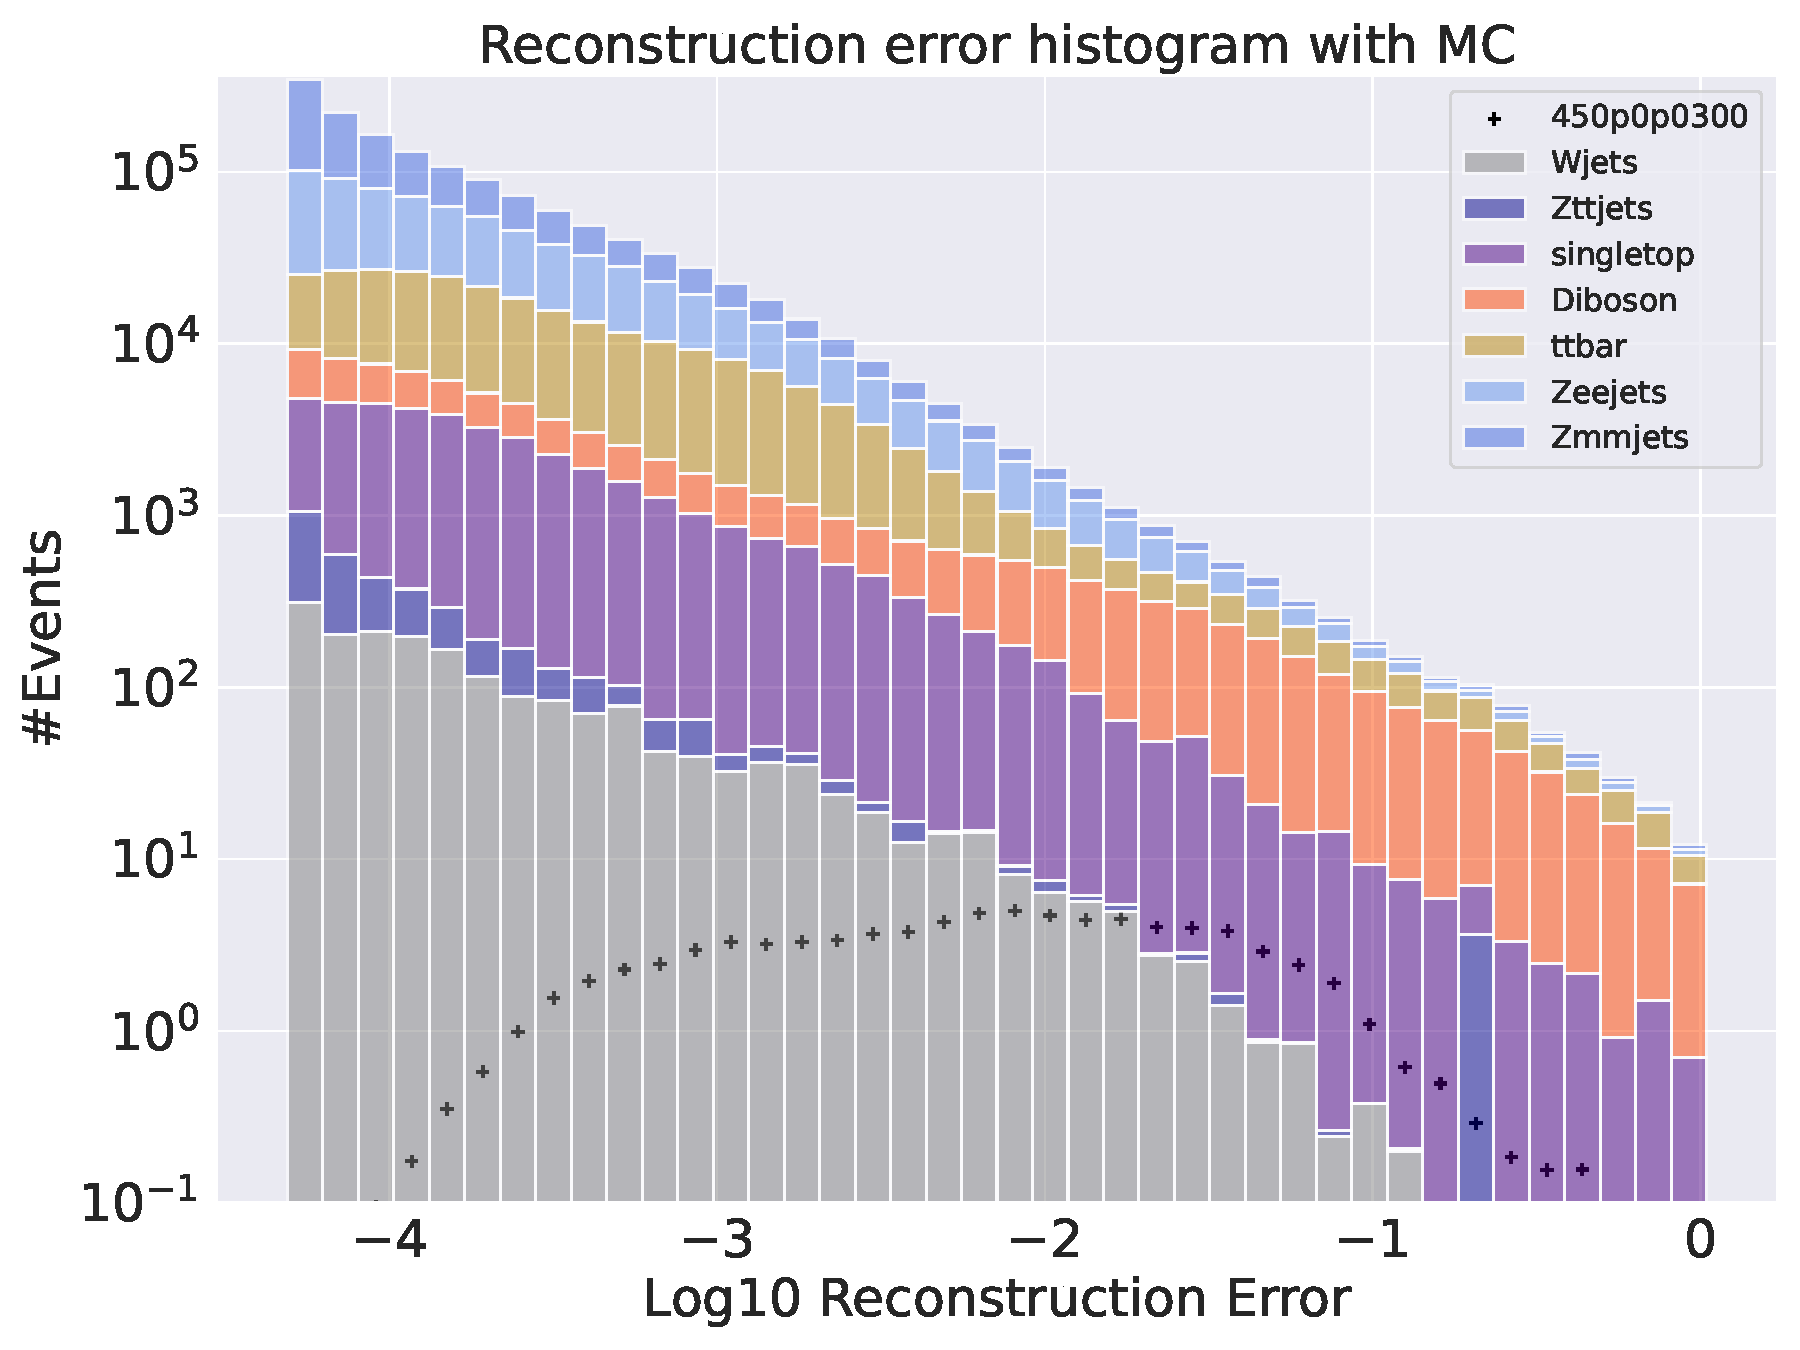
\includegraphics[width=\textwidth]{Figures/AE_testing/small/2lep/b_data_recon_big_rm3_feats_sig_450p0p0300_.pdf}
        \caption{}
        \label{fig:AE_2lep_small_450}
    \end{subfigure}
    \hfill
    \begin{subfigure}{.45\textwidth}
        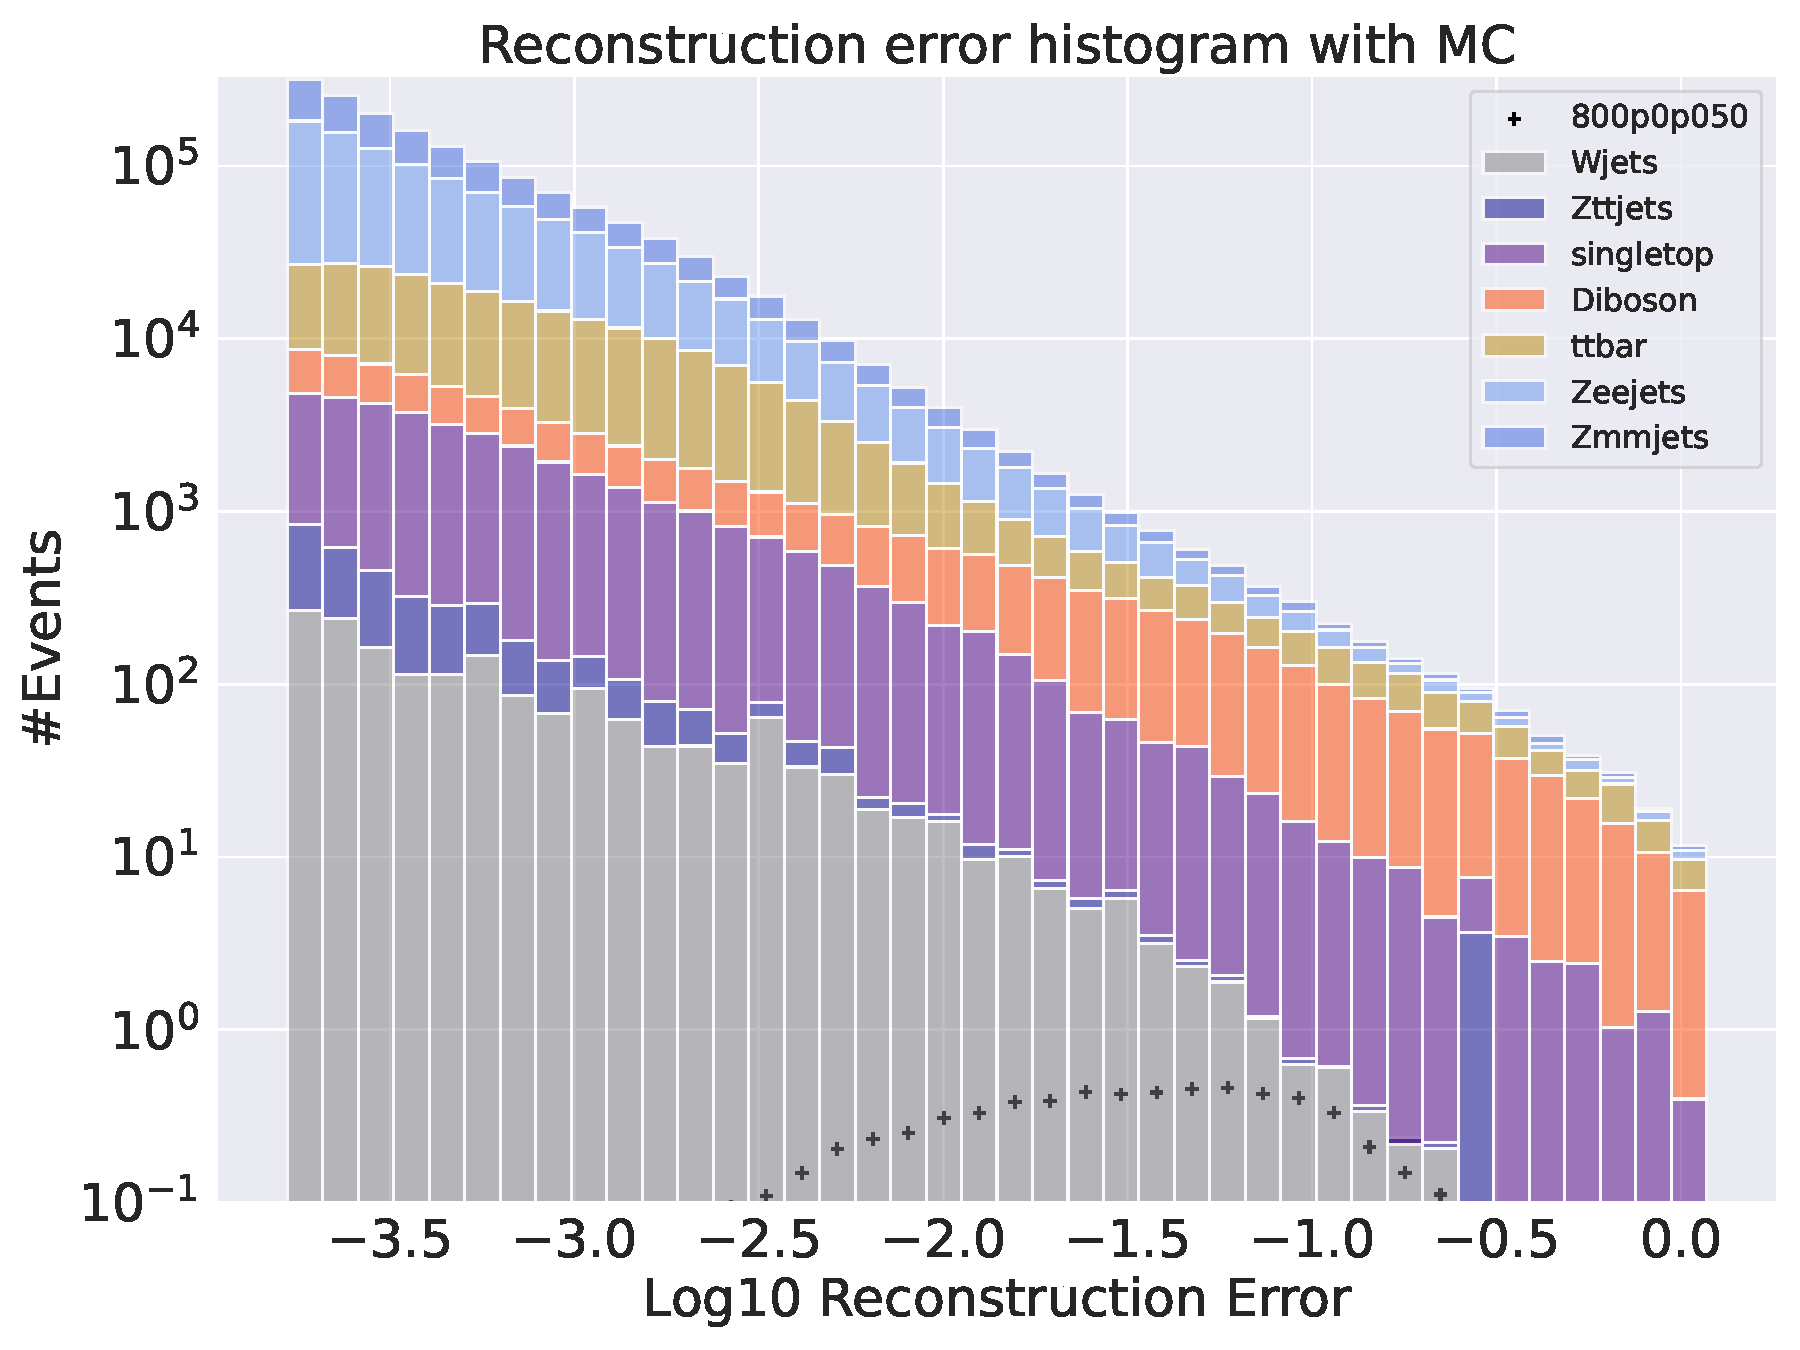
\includegraphics[width=\textwidth]{Figures/AE_testing/big/2lep/b_data_recon_big_rm3_feats_sig_800p0p050_.pdf}
        \caption{}
        \label{fig:AE_2lep_big_800}
    \end{subfigure}
    \hfill   
    \begin{subfigure}{.45\textwidth}
        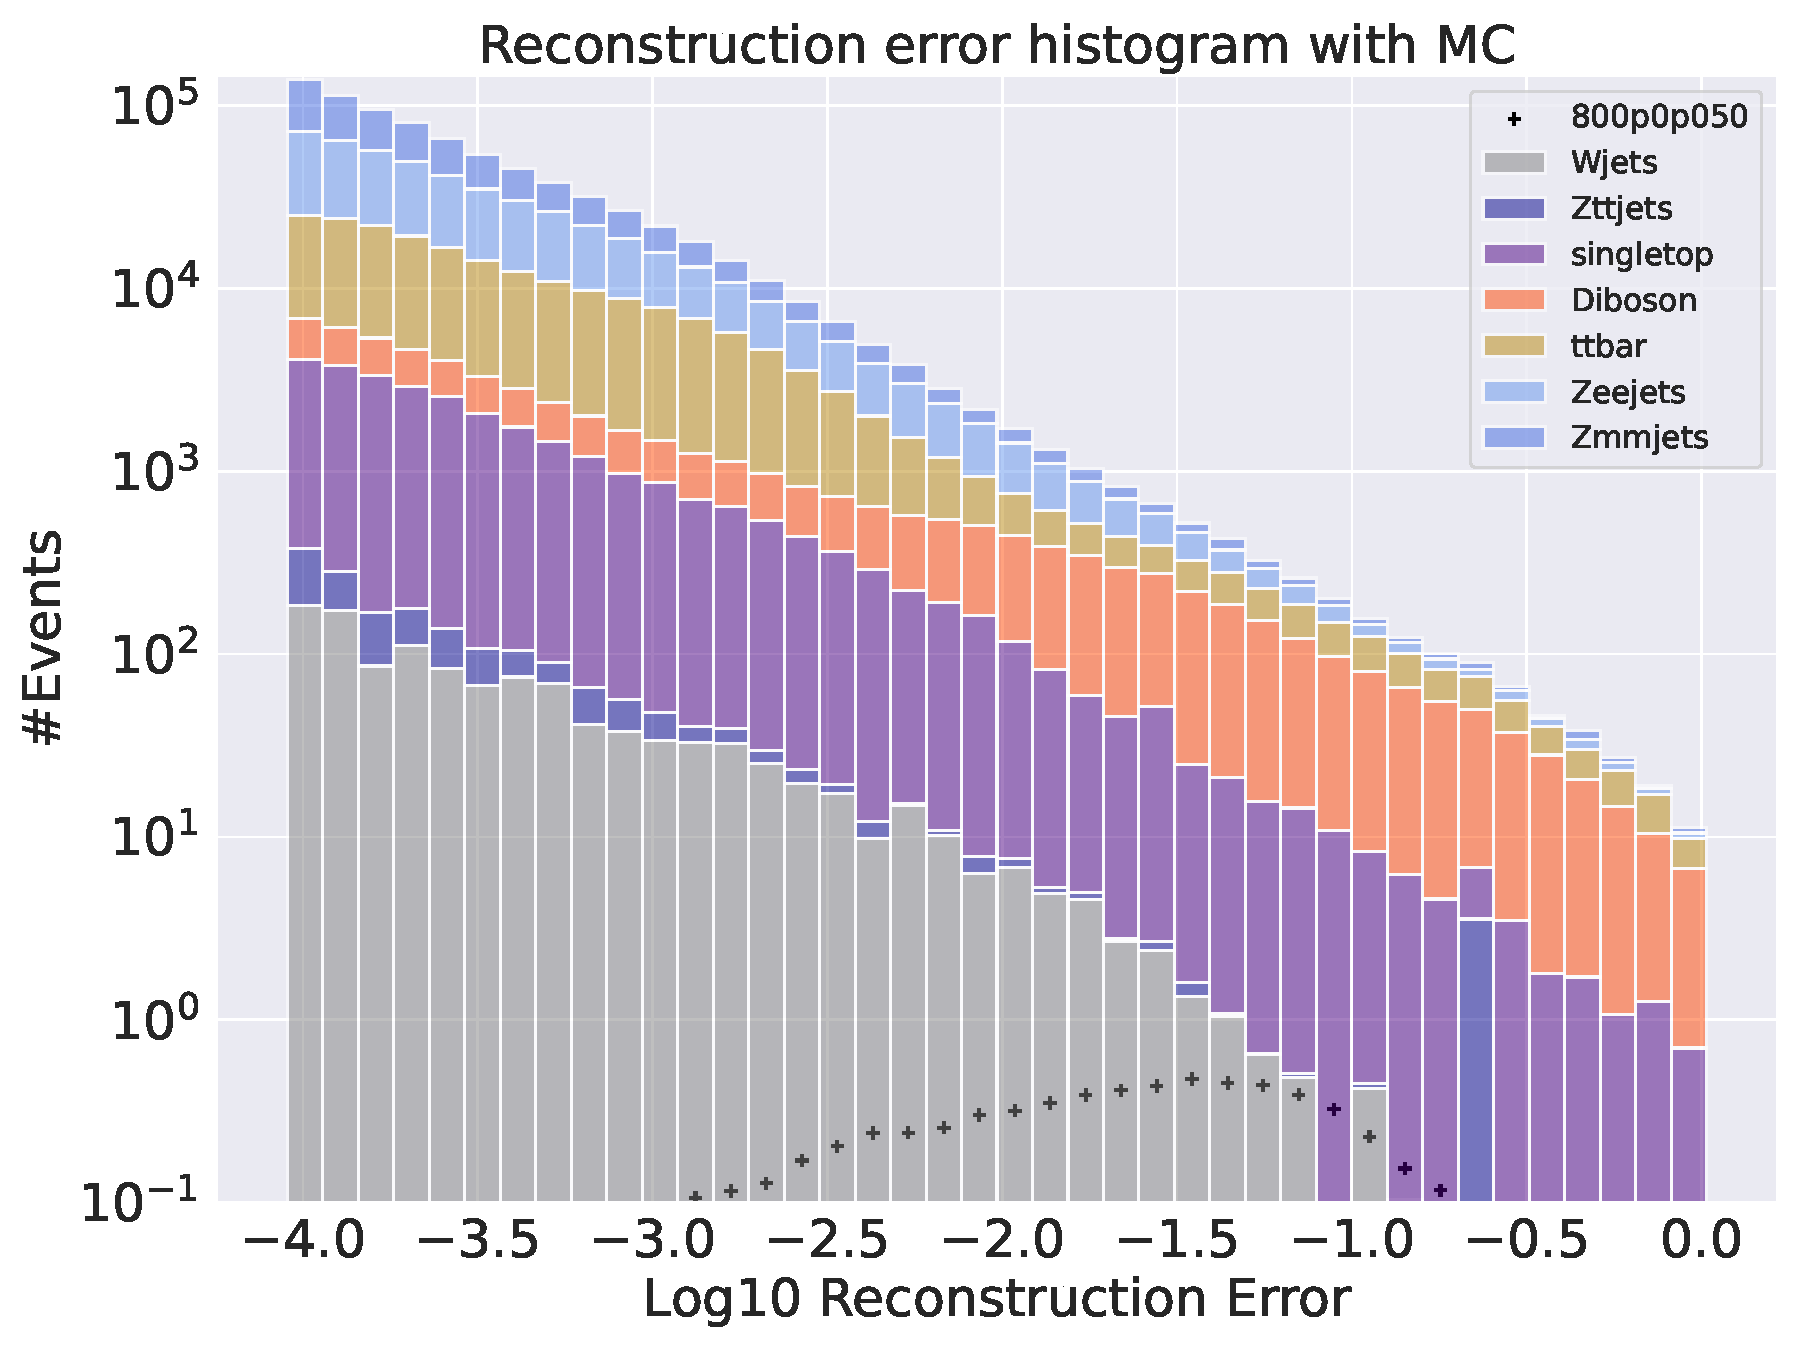
\includegraphics[width=\textwidth]{Figures/AE_testing/small/2lep/b_data_recon_big_rm3_feats_sig_800p0p050_.pdf}
        \caption{}
        \label{fig:AE_2lep_small_800}
    \end{subfigure}
    \hfill      
    \caption[2lep reconstruction error with SUSY signals for AE]{Reconstruction error distribution for the small (left) and large (right)
    regular autoencoder, using the 2 lepton + $e_T^{miss}$ dataset as training and test set. The signals used are the same SUSY signals 
    from the 3 lepton case. Figures \ref{fig:AE_2lep_big_450} and \ref{fig:AE_2lep_small_450} shows the SUSY 450 and 300 mass signal, 
    and figures \ref{fig:AE_2lep_big_800} and \ref{fig:AE_2lep_small_800} shows the SUSY 800 and 50 mass signal.}
    \label{fig:AE_2lep_recon_err_both_sig}
\end{figure}

In figure \ref{fig:AE_2lep_recon_err_both_sig} we have the reconstruction error distributions for the 2 lepton + $e_T^{miss}$ 
dataset for the regular autoencoder models. There is a general trend here for both the small and large regular autoencoder, which is that 
the distribution is highly shifted to the lower end of the reconstruction error range. This is a continuing trend following the 3 lepton + $e_T^{miss}$
showin i figure \ref{fig:ae_susy_450_300_800_50_recon_etmiss}. This indicates that as we increase the statistics, in other words the amount of 
background events, the ability of the autoencoder to learn the internal structure increases. It is also interesting to observe here that 
as the reconstruction error increases, the amount of each sample in a given bin changes alot. As expected, Zmmjets and Zeejets along with 
ttbar are the events with the highest statistics in the 2 lepton + $e_T^{miss}$ dataset, thus it should be easier to learn to better 
reconstruct those events. However, note the amount of Diboson in the higher end of the reconstruction error histograms, as well as in 
the $e_T^{miss}$ post reconstruction error cut distributions. One explanation for this could be the sample discrepencay explained in section
 \ref{sec:mcdatacomp}. It would appear that too much of the diboson samples is cut, leading to not enough samples for it to appropriatly 
 learn the RMM structure for that channel, leading to the high reconstruction error values for some of those events. Note also here that
  the reconstruction threshold where this effet is getting more notisable around $10^{-2}$ and larger, where the events are on the order of 
  a 1000 or less per bin. Thus it is not alot of events, but still enough to note. \par 
Using the signal region definition from above we set cuts on the reconstruction error and then calculate the significance of the signal. 
The figures with the best significance are shown below:

\begin{figure}[H]
    \centering
    \begin{subfigure}{.45\textwidth}
        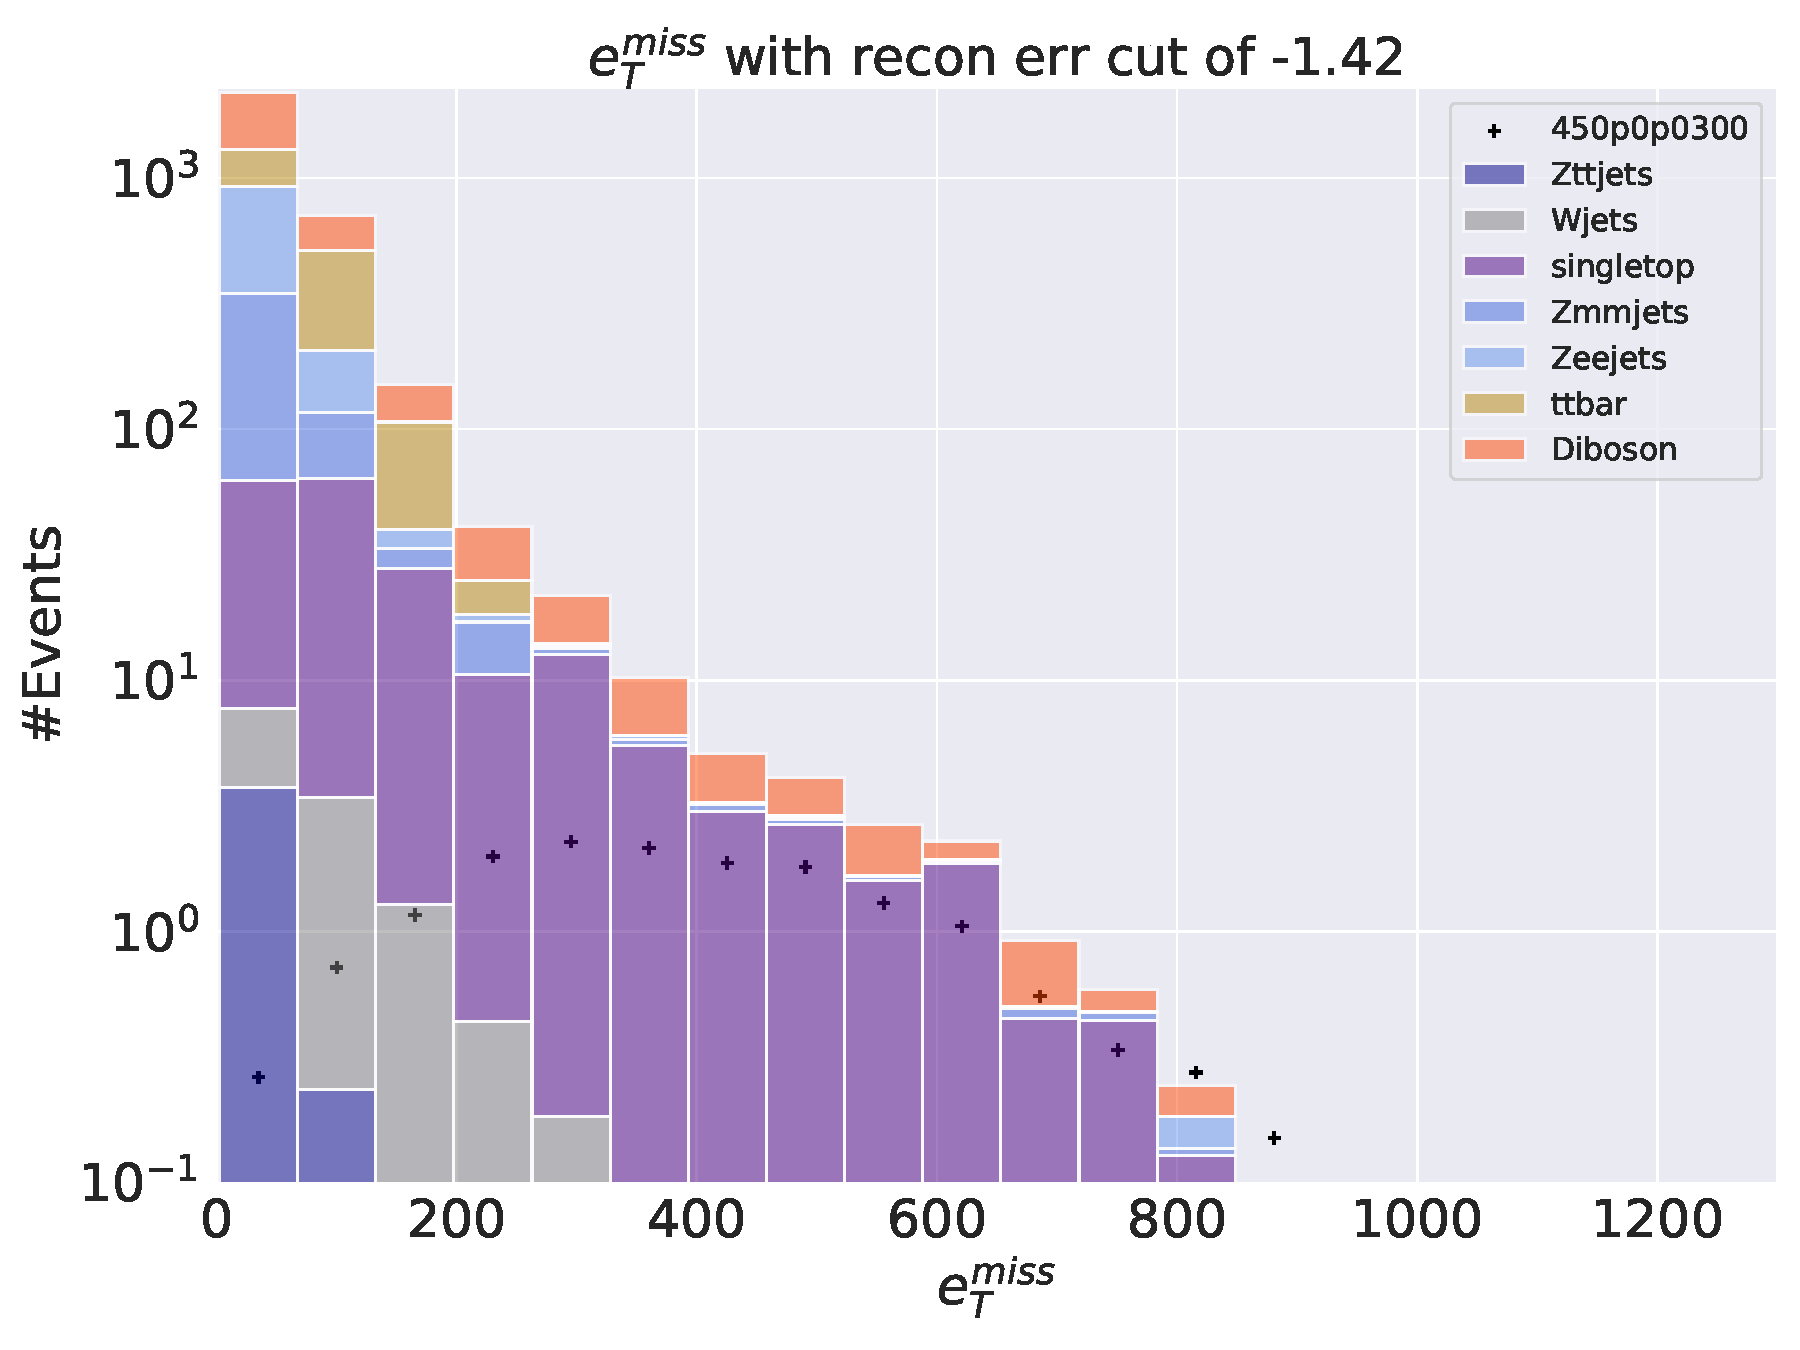
\includegraphics[width=\textwidth]{Figures/AE_testing/big/2lep/b_data_recon_big_rm3_feats_sig_450p0p0300_recon_errcut_-1.42.pdf}
        \caption{ }
        \label{fig:AE_2lep_big_450_cut_etmiss}
    \end{subfigure}
    \hfill
    \begin{subfigure}{.45\textwidth}
        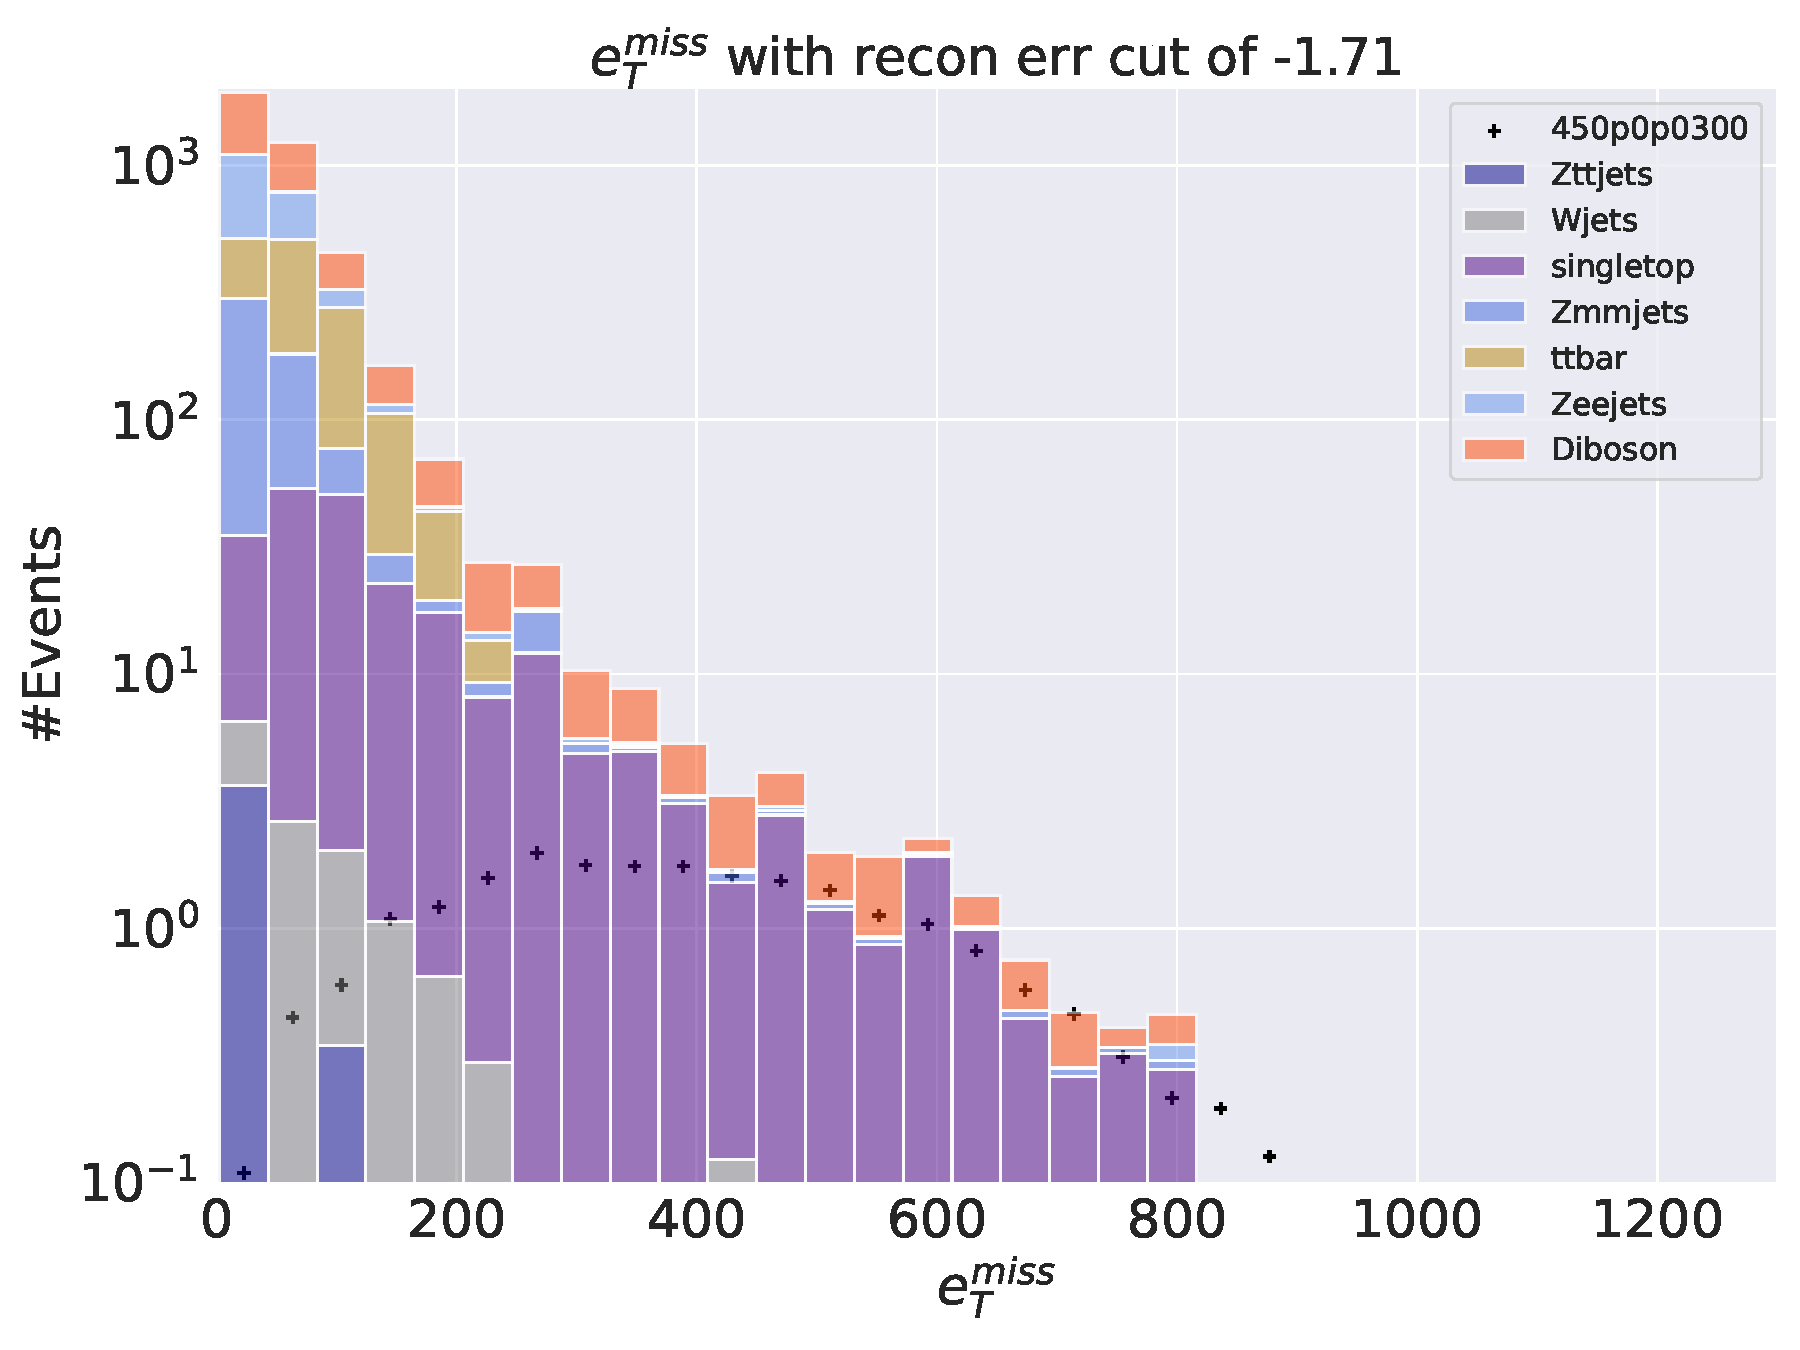
\includegraphics[width=\textwidth]{Figures/AE_testing/small/2lep/b_data_recon_big_rm3_feats_sig_450p0p0300_recon_errcut_-1.71.pdf}
        \caption{}
        \label{fig:AE_2lep_small_450_cut_etmiss}
    \end{subfigure}
    \hfill
    \begin{subfigure}{.45\textwidth}
        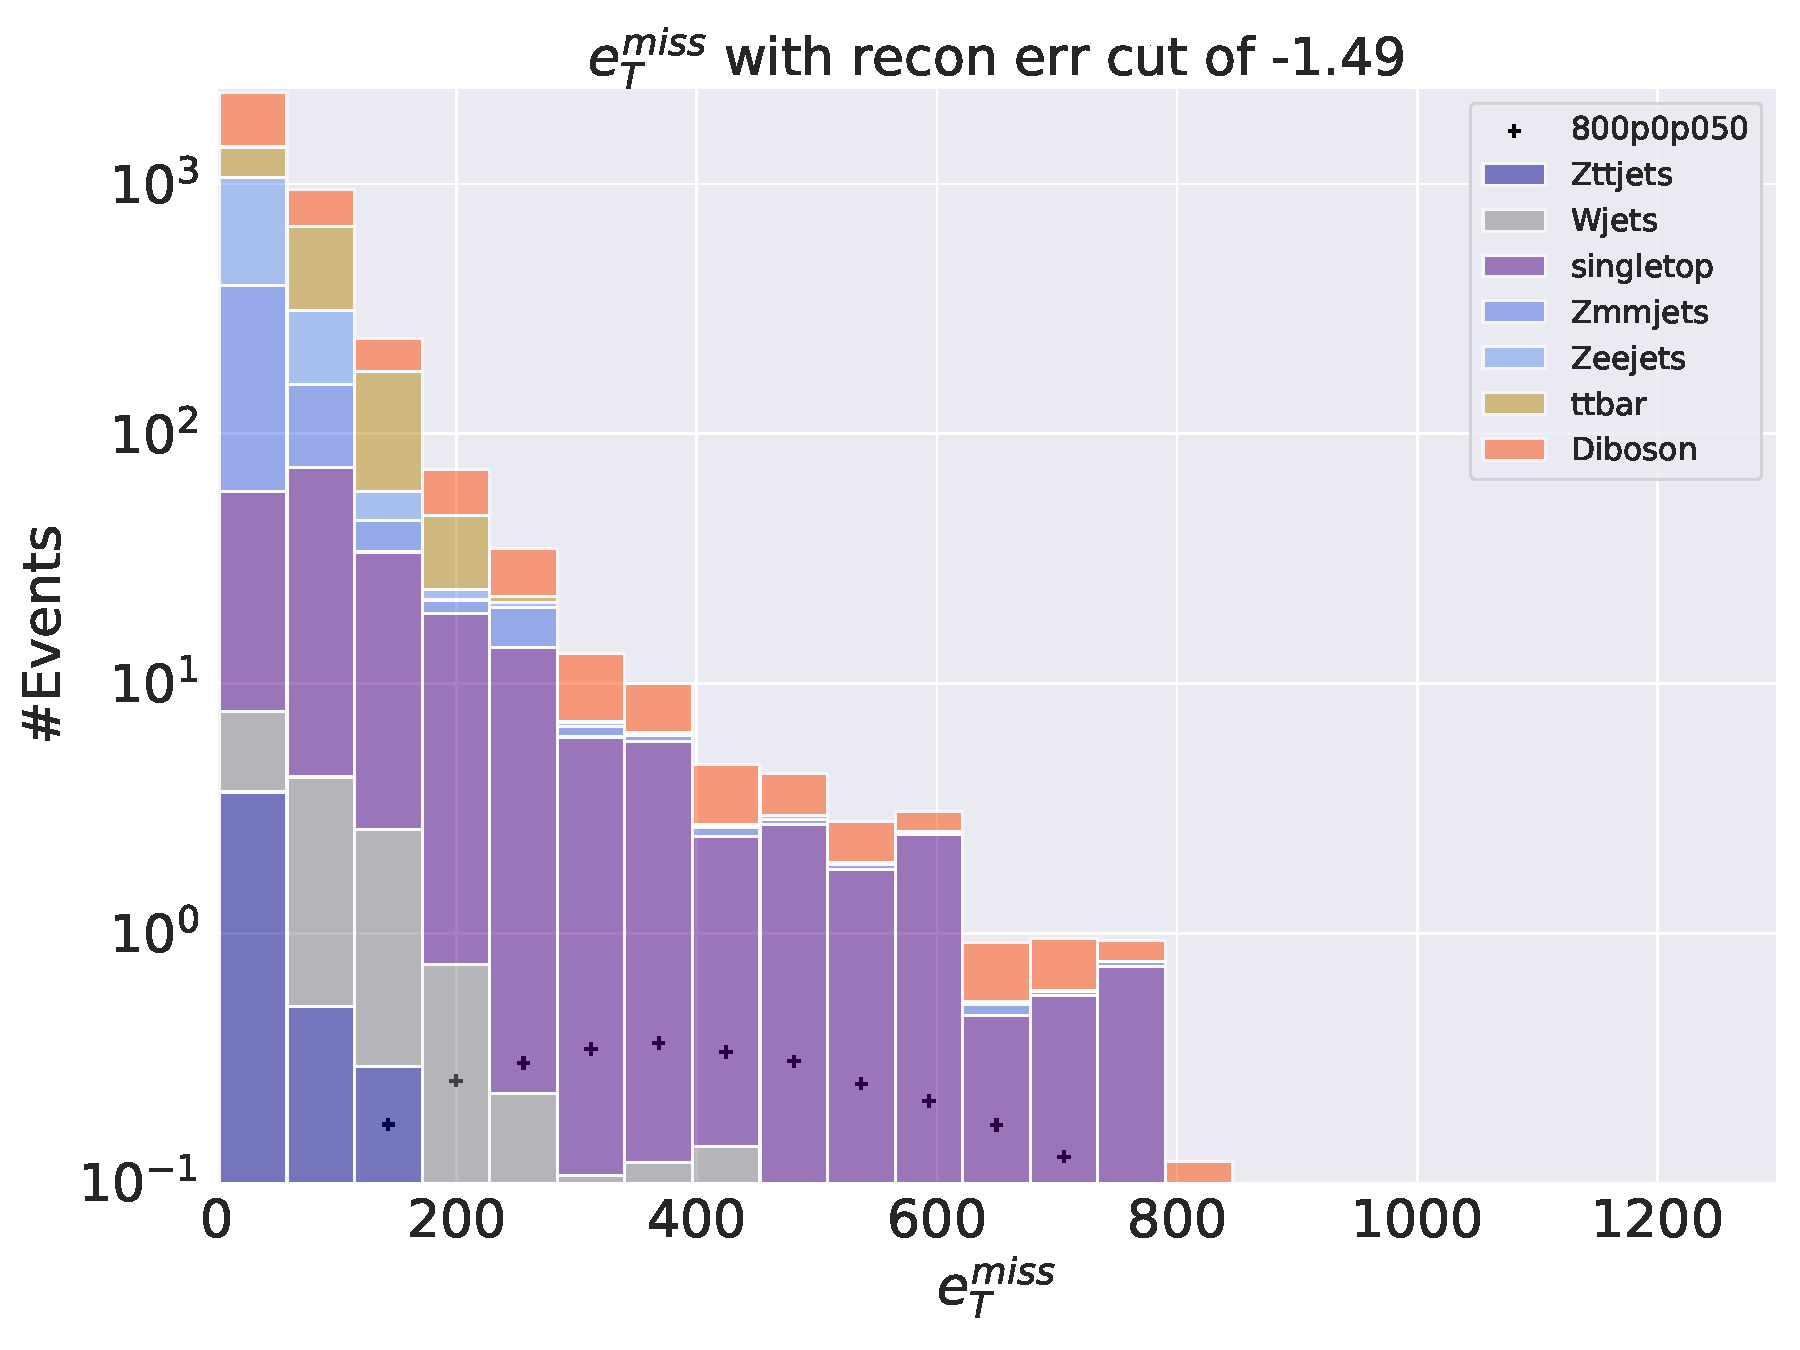
\includegraphics[width=\textwidth]{Figures/AE_testing/big/2lep/b_data_recon_big_rm3_feats_sig_800p0p050_recon_errcut_-1.49.pdf}
        \caption{}
        \label{fig:AE_2lep_big_800_cut_etmiss}
    \end{subfigure}
    \hfill   
    \begin{subfigure}{.45\textwidth}
        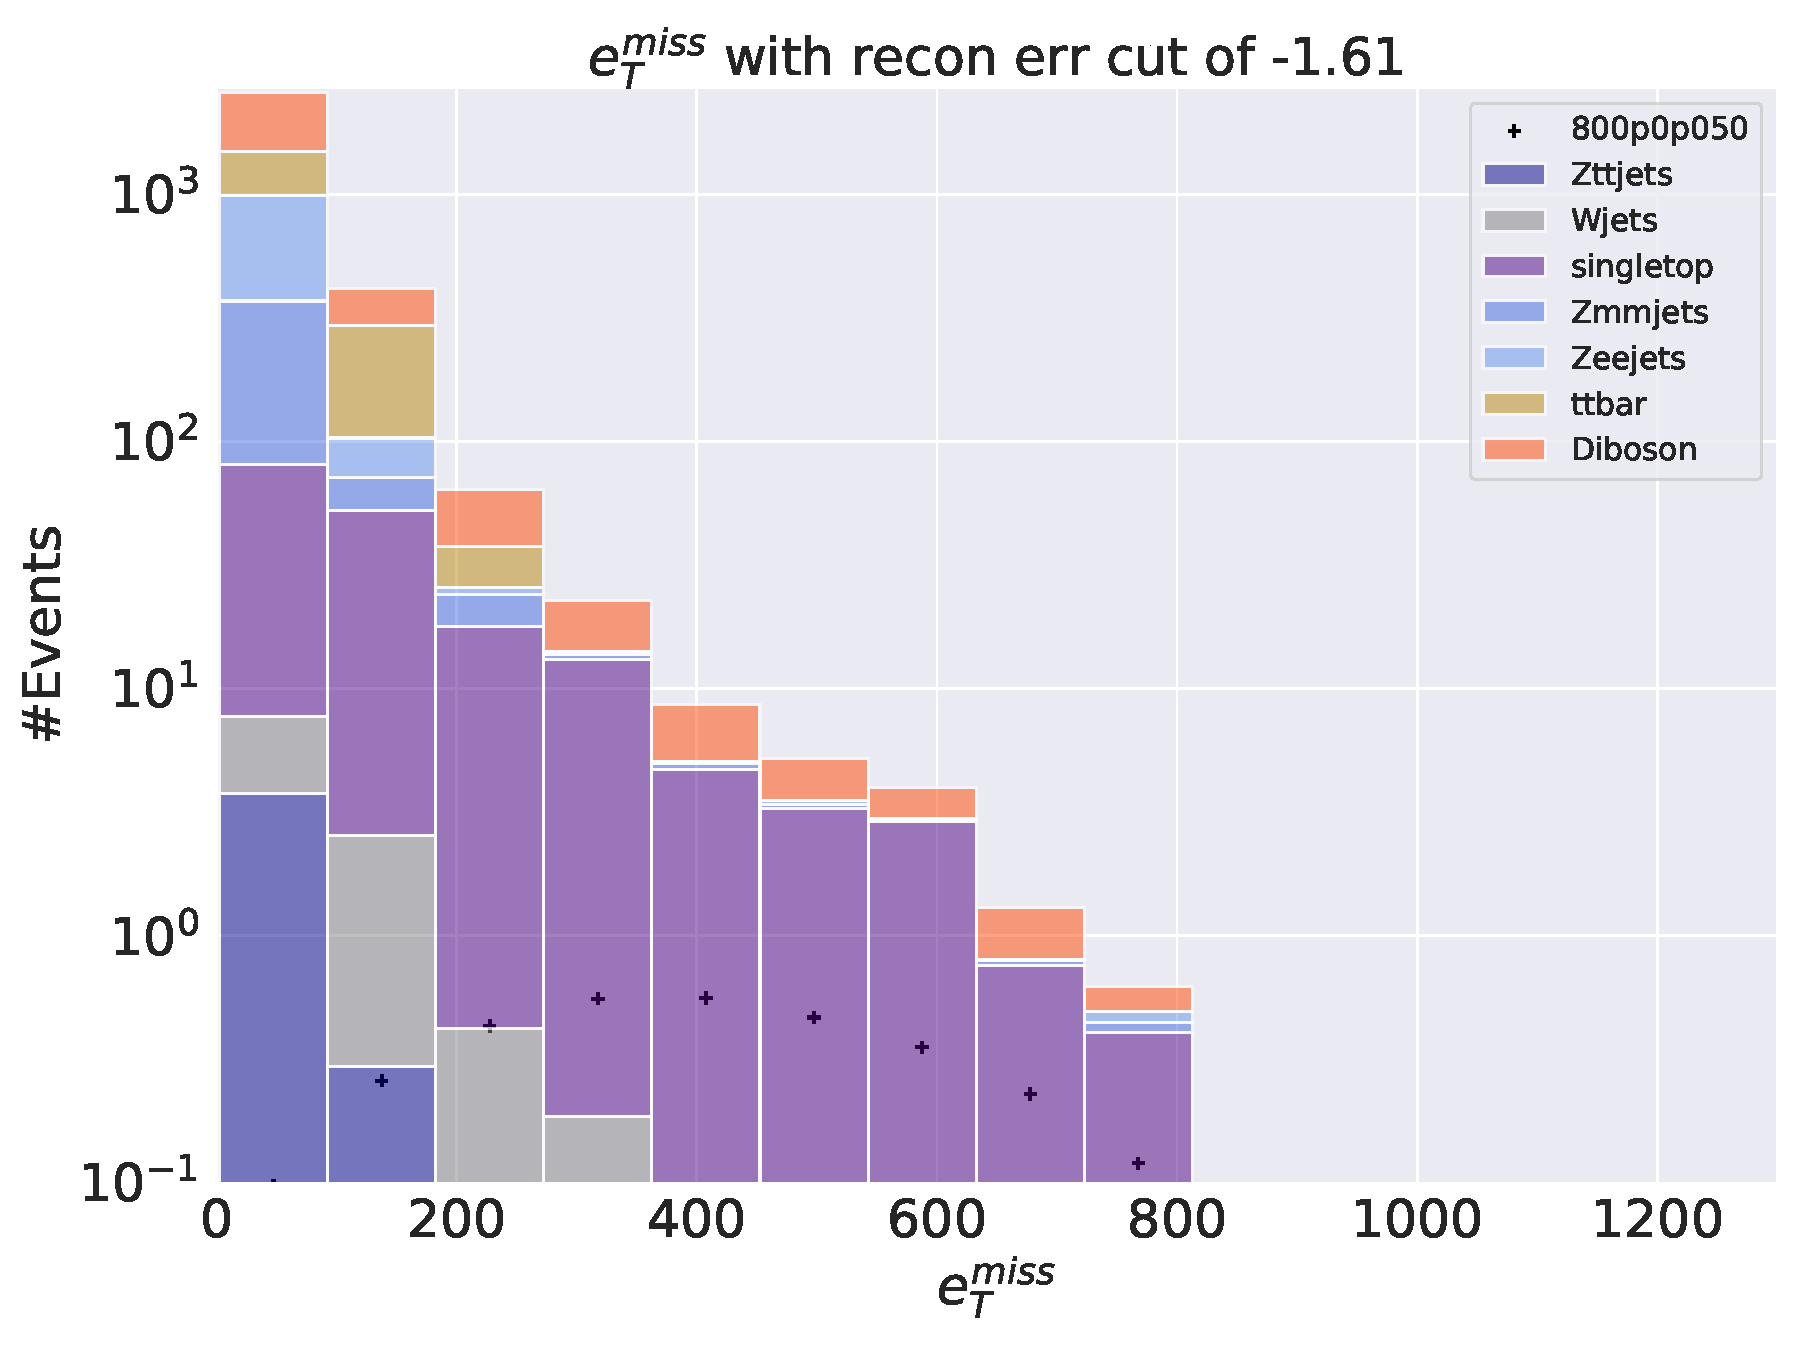
\includegraphics[width=\textwidth]{Figures/AE_testing/small/2lep/b_data_recon_big_rm3_feats_sig_800p0p050_recon_errcut_-1.61.pdf}
        \caption{}
        \label{fig:AE_2lep_small_800_cut_etmiss}
    \end{subfigure}
    \hfill      
    \caption[$e_T^{miss}$ best cuts for regular autoencoder]{$e_T^{miss}$ distribution for small (left) and large (right) autoencoder.
    Each figure used the best cut of three possibilities, the remainding results are in the appendix. By best, it is meant that the cut
    gave the best significance. Figures \ref{fig:AE_2lep_big_450} and \ref{fig:AE_2lep_small_450} shows the SUSY 450 and 300 mass signal, 
    and figures \ref{fig:AE_2lep_big_800} and \ref{fig:AE_2lep_small_800} shows the SUSY 800 and 50 mass signal.}
    \label{fig:AE_2lep_recon_err_both_sig_cut_etmiss}
\end{figure}

In figure \ref{fig:AE_2lep_recon_err_both_sig_cut_etmiss} we have the $e_T^{miss}$ distributions for the best cuts for the regular autoencoder models.
The cuts then gives rise to the significance for each signal region. Now, one indication that the method could work is if the models can improve the 
significance from just looking at the $e_T^{miss}$ distributions of the background and the signal in mind. The significances corresponding to each 
reconstruction error cuts are all listed below. Note here that for $e_T^{miss}$, no physics basedcuts have been used, but there are certain cuts 
that can increase the significance, so the results in the following table should be thought carefully of.

\begin{table}[H]
    \centering
    \caption[Significance table regular autoencoder]{Significance table for the regular autoencoder models. For each signal for both the small and 
    large regular autoencoder, the significance is calculated with equation small (left column) and equation large (right column). The 
    reconstruction error cuts used where $[-1.42, -1.07, -0.71]$ for the SUSY $450p300$ signal and $[-1.49, -1.11, -0.74]$ for the SUSY 
    $800p50$ signal for the large autoencoder. The reconstruction error cuts used for the small autoencoder where $[-1.71, -1.29, -0.86]$ 
    for the SUSY $450p300$ signal and $[-1.61, -1.21, -0.81]$ for the SUSY $800p50$ signal. }
    \label{tab:AE_2lep_significance}
    \begin{tabular}{|llllllll|}
    \hline
    \multicolumn{8}{|c|}{Regular Autoencoder}                                                                                                                                    \\ \hline
    \multicolumn{4}{|c|}{Small}                                                                    & \multicolumn{4}{c|}{Large}                                                  \\ \hline
    \multicolumn{2}{|l|}{450p300}                  & \multicolumn{2}{l|}{800p50}                   & \multicolumn{2}{l|}{450p300}                  & \multicolumn{2}{l|}{800p50} \\ \hline
    \multicolumn{8}{|c|}{Pre reconstruction error cut significance}                                                                                                                           \\ \hline
    \multicolumn{1}{|l|}{0.35} & \multicolumn{1}{l|}{0.02} & \multicolumn{1}{l|}{$NaN$} & \multicolumn{1}{l|}{0.002} & \multicolumn{1}{l|}{0.35} & \multicolumn{1}{l|}{0.02} & \multicolumn{1}{l|}{$NaN$}  & \multicolumn{1}{l|}{0.002} \\ \hline
    \multicolumn{8}{|c|}{Post reconstruction error  cut significance}                                                                                                                         \\ \hline
    \multicolumn{1}{|l|}{0.35} & \multicolumn{1}{l|}{0.35} & \multicolumn{1}{l|}{0.06} & \multicolumn{1}{l|}{0.06} & \multicolumn{1}{l|}{0.29} & \multicolumn{1}{l|}{0.29} & \multicolumn{1}{l|}{0.05}   & \multicolumn{1}{l|}{0.05}  \\ \hline
    \multicolumn{1}{|l|}{0.20} & \multicolumn{1}{l|}{0.2} & \multicolumn{1}{l|}{0.04} & \multicolumn{1}{l|}{0.04} & \multicolumn{1}{l|}{0.14} & \multicolumn{1}{l|}{0.14} & \multicolumn{1}{l|}{0.04}   & \multicolumn{1}{l|}{0.04}  \\ \hline
    \multicolumn{1}{|l|}{0.06} & \multicolumn{1}{l|}{0.06} & \multicolumn{1}{l|}{0.02} & \multicolumn{1}{l|}{0.02} & \multicolumn{1}{l|}{0.06} & \multicolumn{1}{l|}{0.06} & \multicolumn{1}{l|}{0.02}   & \multicolumn{1}{l|}{0.02} \\ \hline
    \end{tabular}
\end{table}

In table \ref{tab:AE_2lep_significance} we have the small data and large data significance on $e_T^{miss}$ for both the small and large regular autoencoder models,
calculated for both the SUSY $450p300$ and $800p50$ models. The table compares the pre reconstruction error significance with post reconstruction error significance. 
Note that the significance have been rounded up to two decimals, and the actual values with 17 decimal precision can be found in the $significance\_MODELTYPE\_MODELSIZE.txt$ 
in the codebase folder in github: \href{https://github.com/Gadangadang/MasterThesis/tree/main/CodeBase/Analysis}{$MasterThesis/tree/main/CodeBase/Analysis$}. MODELTYPE 
refers to the type of autoencoder, either AE for regular autoencoder, or VAE for variational autoencoder. MODELSIZE refers to the size of the autoencoder, either small 
for the shallow model, or big for the deep model. \par 
First, it should be noted that the significance for the $800p50$ signal model is a lot smaller than for the $450p300$ signal model, even though the separation shown in 
figures \ref{fig:AE_2lep_recon_err_both_sig} and \ref{fig:AE_2lep_recon_err_both_sig_cut_etmiss} would suggest otherwise. All though the peak in both signal models are 
fairly separated from the peak of the SM MC, the SUSY $800p50$ signal model is shifted a lot more. This is consistant with expectation, as that specific signal model 
has a lot of missing transverse energy, compared to even the other SUSY signal model. Now, The reason for the low significance is most likely the fact that the signal sample 
contains low statistics, in other words, the weights are just a lot lower, compared to the other signal sample. We also have to cases where the significance is $NaN$. 
This only happens in the case we use equation \ref{eq:significance_small}, and is either because the square root has a negative term inside it, or because the logarithm 
has a negative term inside it. \par

From figure \ref{fig:VAE_2lep_recon_err_both_sig} below we have the variational autoencoder output for the 2 lepton case. 

\begin{figure}[H]
    \centering
    \begin{subfigure}{.45\textwidth}
        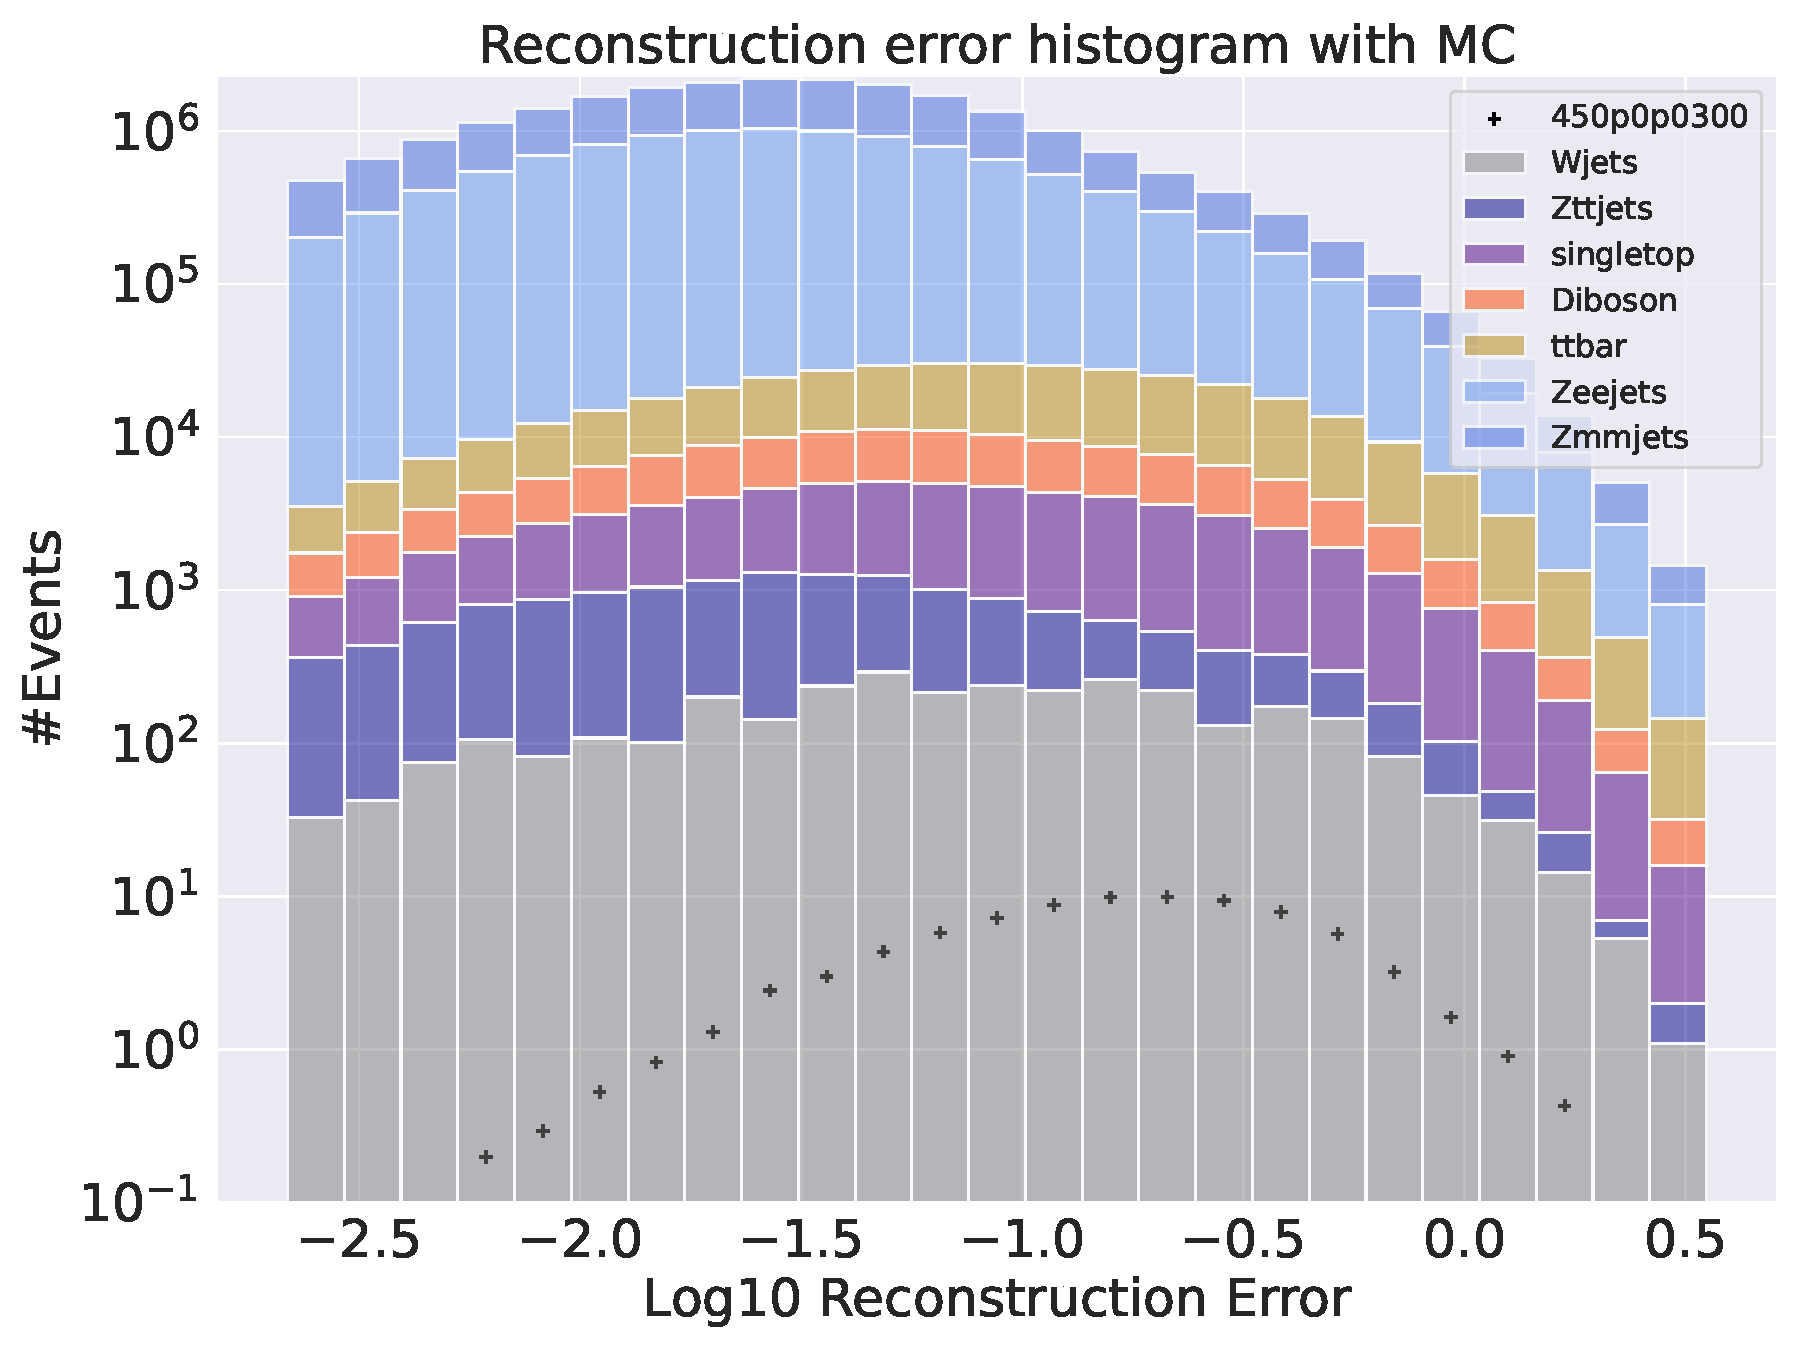
\includegraphics[width=\textwidth]{Figures/VAE_testing/big/2lep/b_data_recon_big_rm3_feats_sig_450p0p0300_.pdf}
        \caption{ }
        \label{fig:VAE_2lep_big_450}
    \end{subfigure}
    \hfill
    \begin{subfigure}{.45\textwidth}
        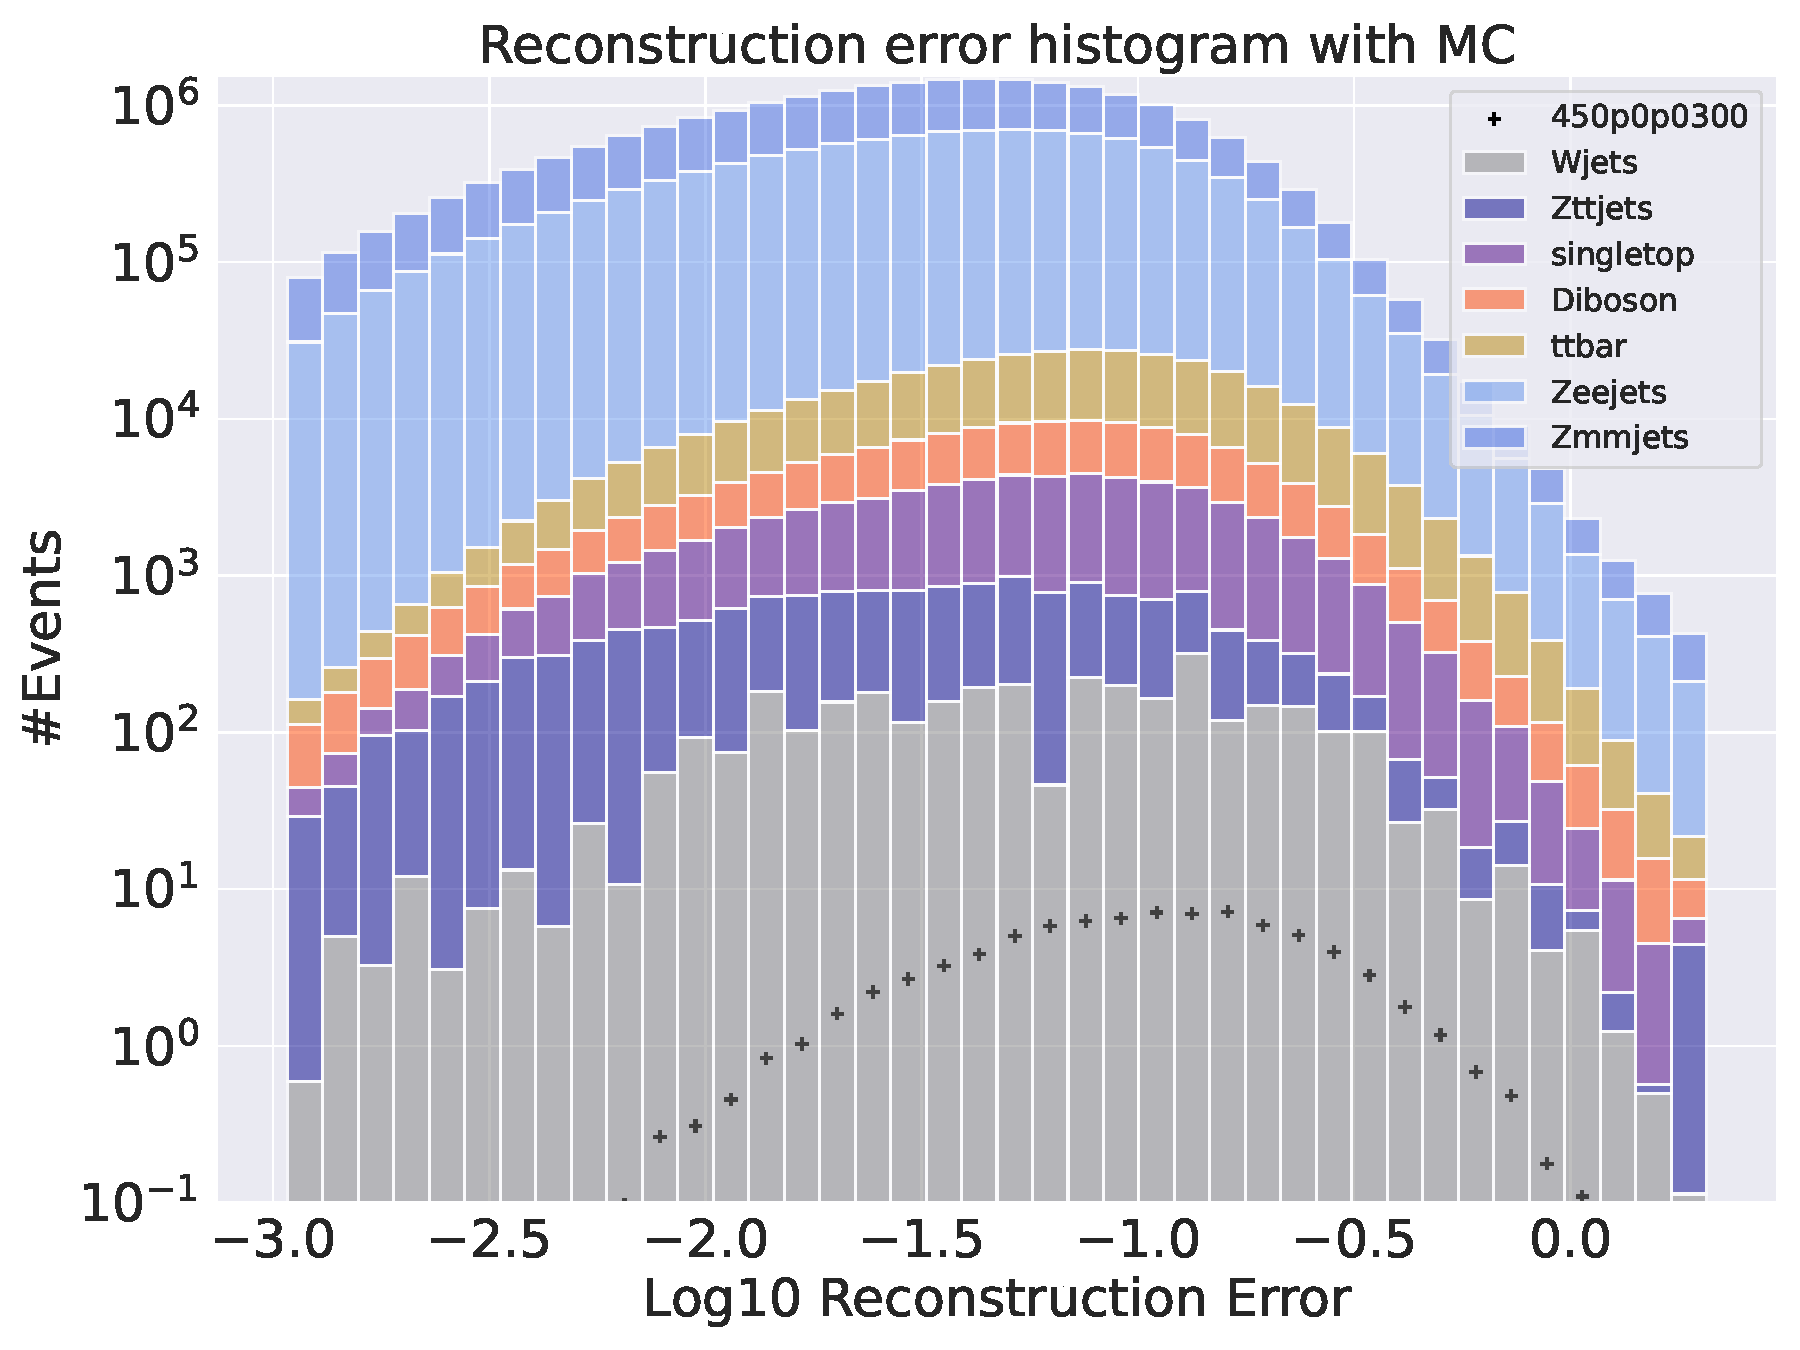
\includegraphics[width=\textwidth]{Figures/VAE_testing/small/2lep/b_data_recon_big_rm3_feats_sig_450p0p0300_.pdf}
        \caption{}
        \label{fig:VAE_2lep_small_450}
    \end{subfigure}
    \hfill
    \begin{subfigure}{.45\textwidth}
        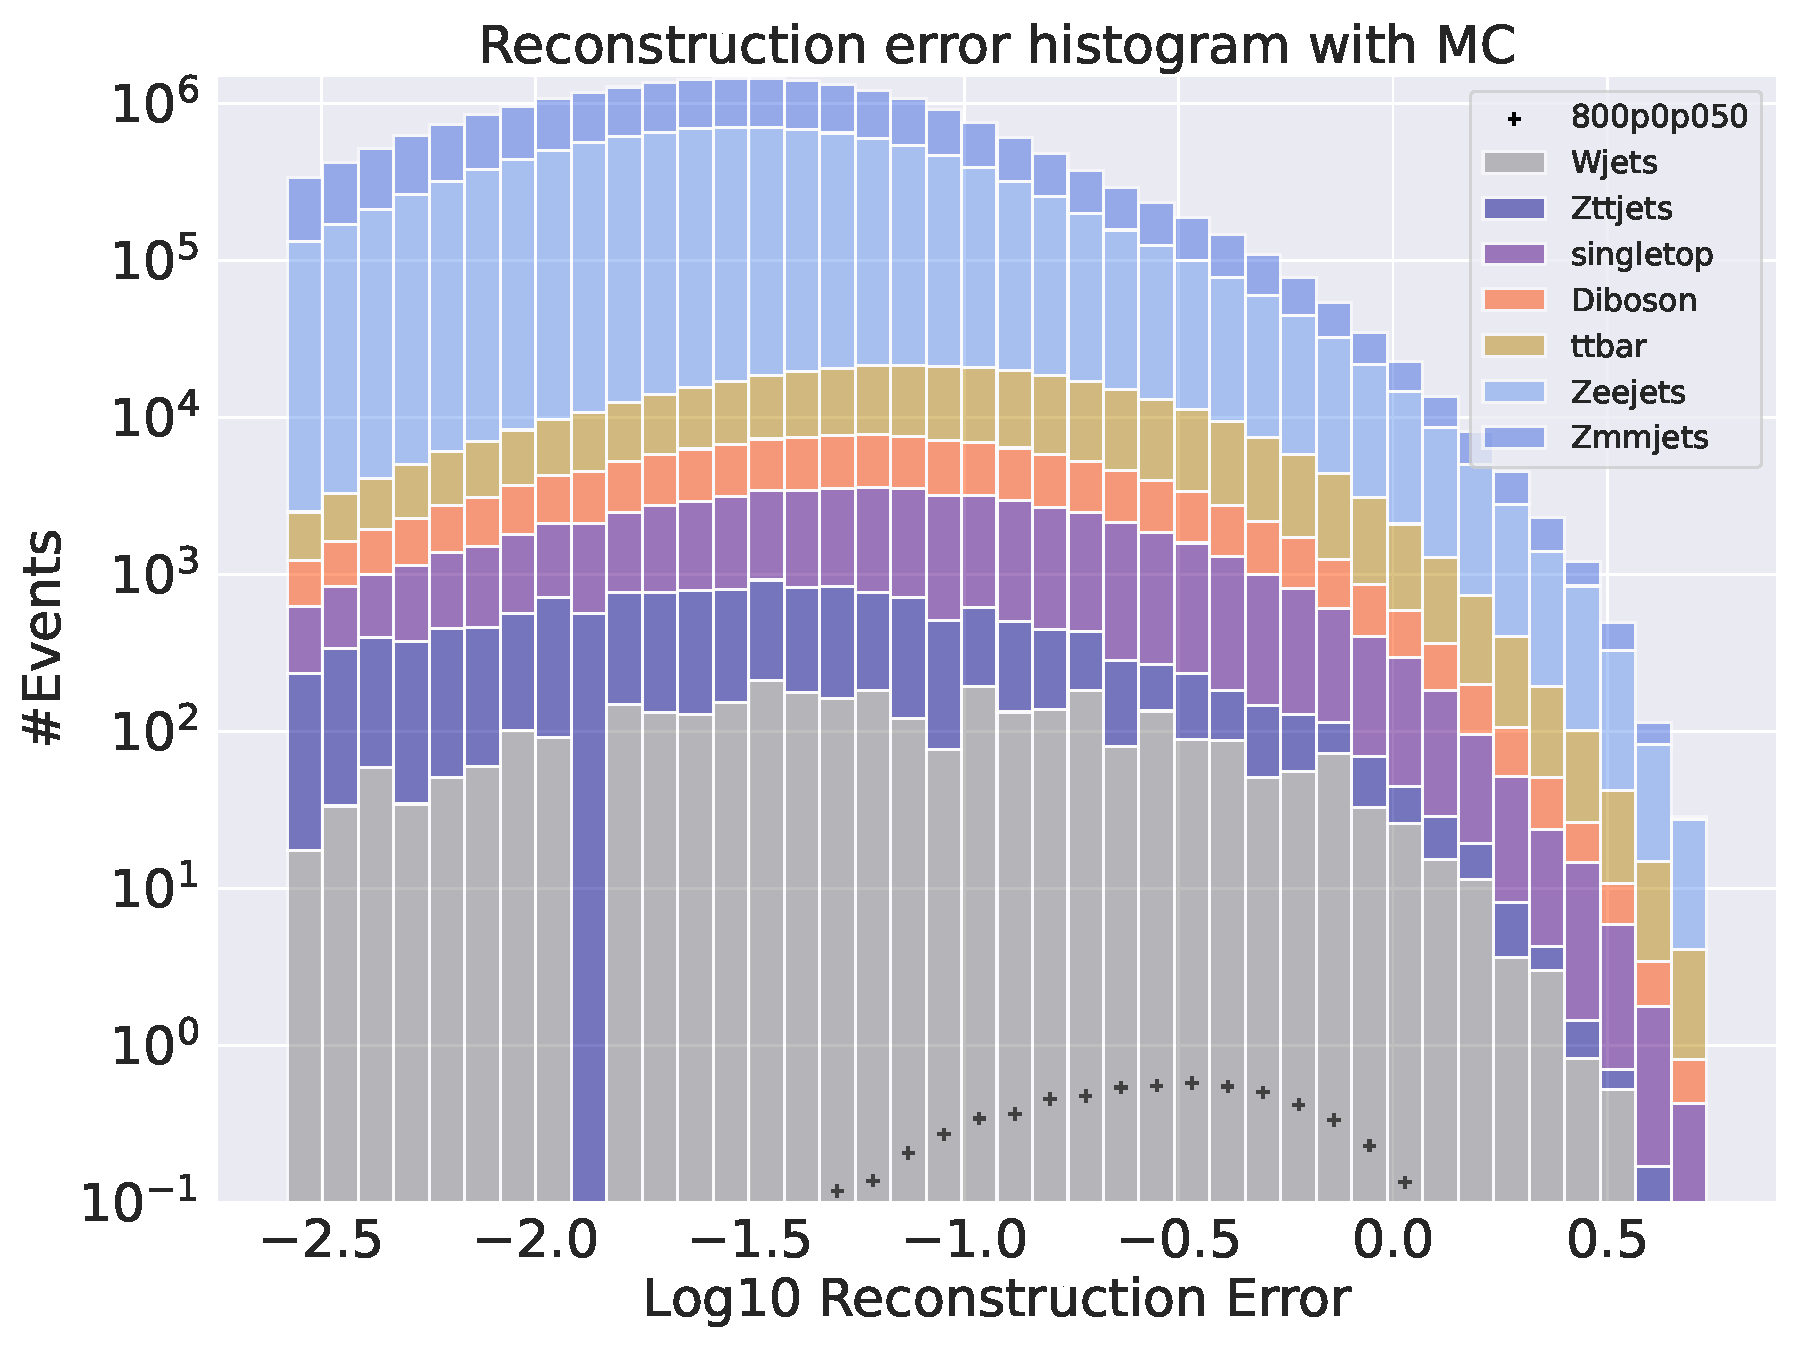
\includegraphics[width=\textwidth]{Figures/VAE_testing/big/2lep/b_data_recon_big_rm3_feats_sig_800p0p050_.pdf}
        \caption{}
        \label{fig:VAE_2lep_big_800}
    \end{subfigure}
    \hfill   
    \begin{subfigure}{.45\textwidth}
        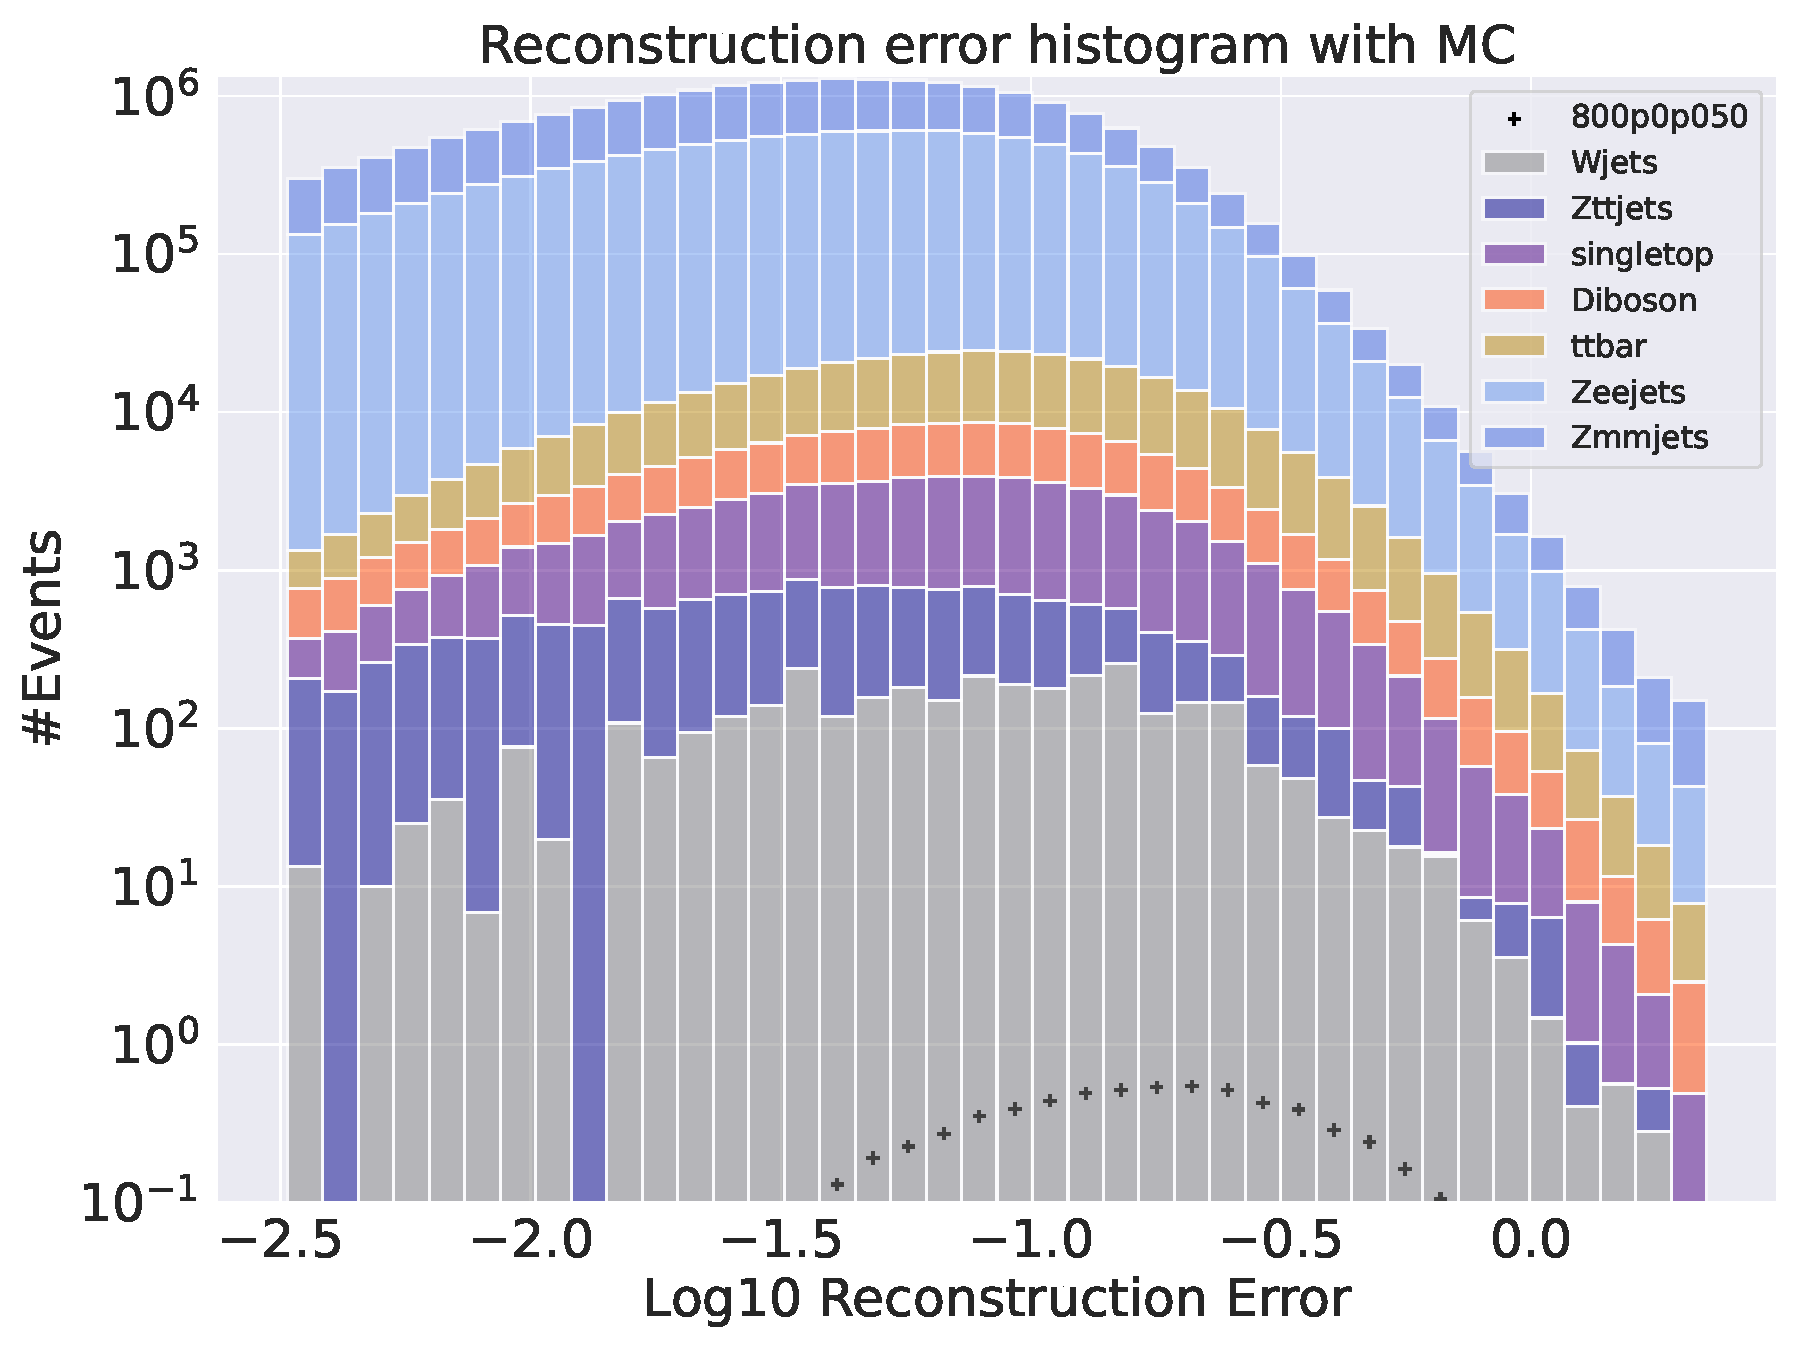
\includegraphics[width=\textwidth]{Figures/VAE_testing/small/2lep/b_data_recon_big_rm3_feats_sig_800p0p050_.pdf}
        \caption{}
        \label{fig:VAE_2lep_small_800}
    \end{subfigure}
    \hfill      
    \caption[2lep reconstruction error with SUSY signals for VAE]{Reconstruction error distribution for the small (left) and large (right)
    regular autoencoder, using the 2 lepton + $e_T^{miss}$ dataset as training and test set. The signals used are the same SUSY signals 
    from the 3 lepton case. Figures \ref{fig:VAE_2lep_big_450} and \ref{fig:VAE_2lep_small_450} shows the SUSY 450 and 300 mass signal, 
    and figures \ref{fig:VAE_2lep_big_800} and \ref{fig:VAE_2lep_small_800} shows the SUSY 800 and 50 mass signal.}
    \label{fig:VAE_2lep_recon_err_both_sig}
\end{figure}

In figure \ref{fig:VAE_2lep_recon_err_both_sig} we have the reconstruction error distributions for both SUSY signals for 
the small and large variational autoencoder. Here we observe that the peak of the distributions for the SM MC in all four cases 
are somewhat centered in the middle of the reconstruction error range, which differs from the steep slope we saw in figure
\ref{fig:AE_2lep_recon_err_both_sig}. Interestingly, we see here that the deepness of the neural network here plays a role, 
which is different from the regular autoencoder output, where both the small and large autoencoder made a steep slope shape of 
the SM MC reconstruction error distribution. The peak of the distribution here is slightly shifted to the left for the shallow 
autoencoder model, and slightly shifted to the right of the center with the deep autoencoder model. One possible reason for this 
somewhat Gaussian like distribution could be that the variational autoencoder, via the reparametization trick from section 
\ref{sec:reparameterization}, samples from a Gaussian distribution that has yet to be trained on enough data to produce a 
good enough error distribution. It could also be that the batch size is too large, and that the model has to train on smaller 
batches to get a better result. 

\begin{figure}[H]
    \centering
    \begin{subfigure}{.45\textwidth}
        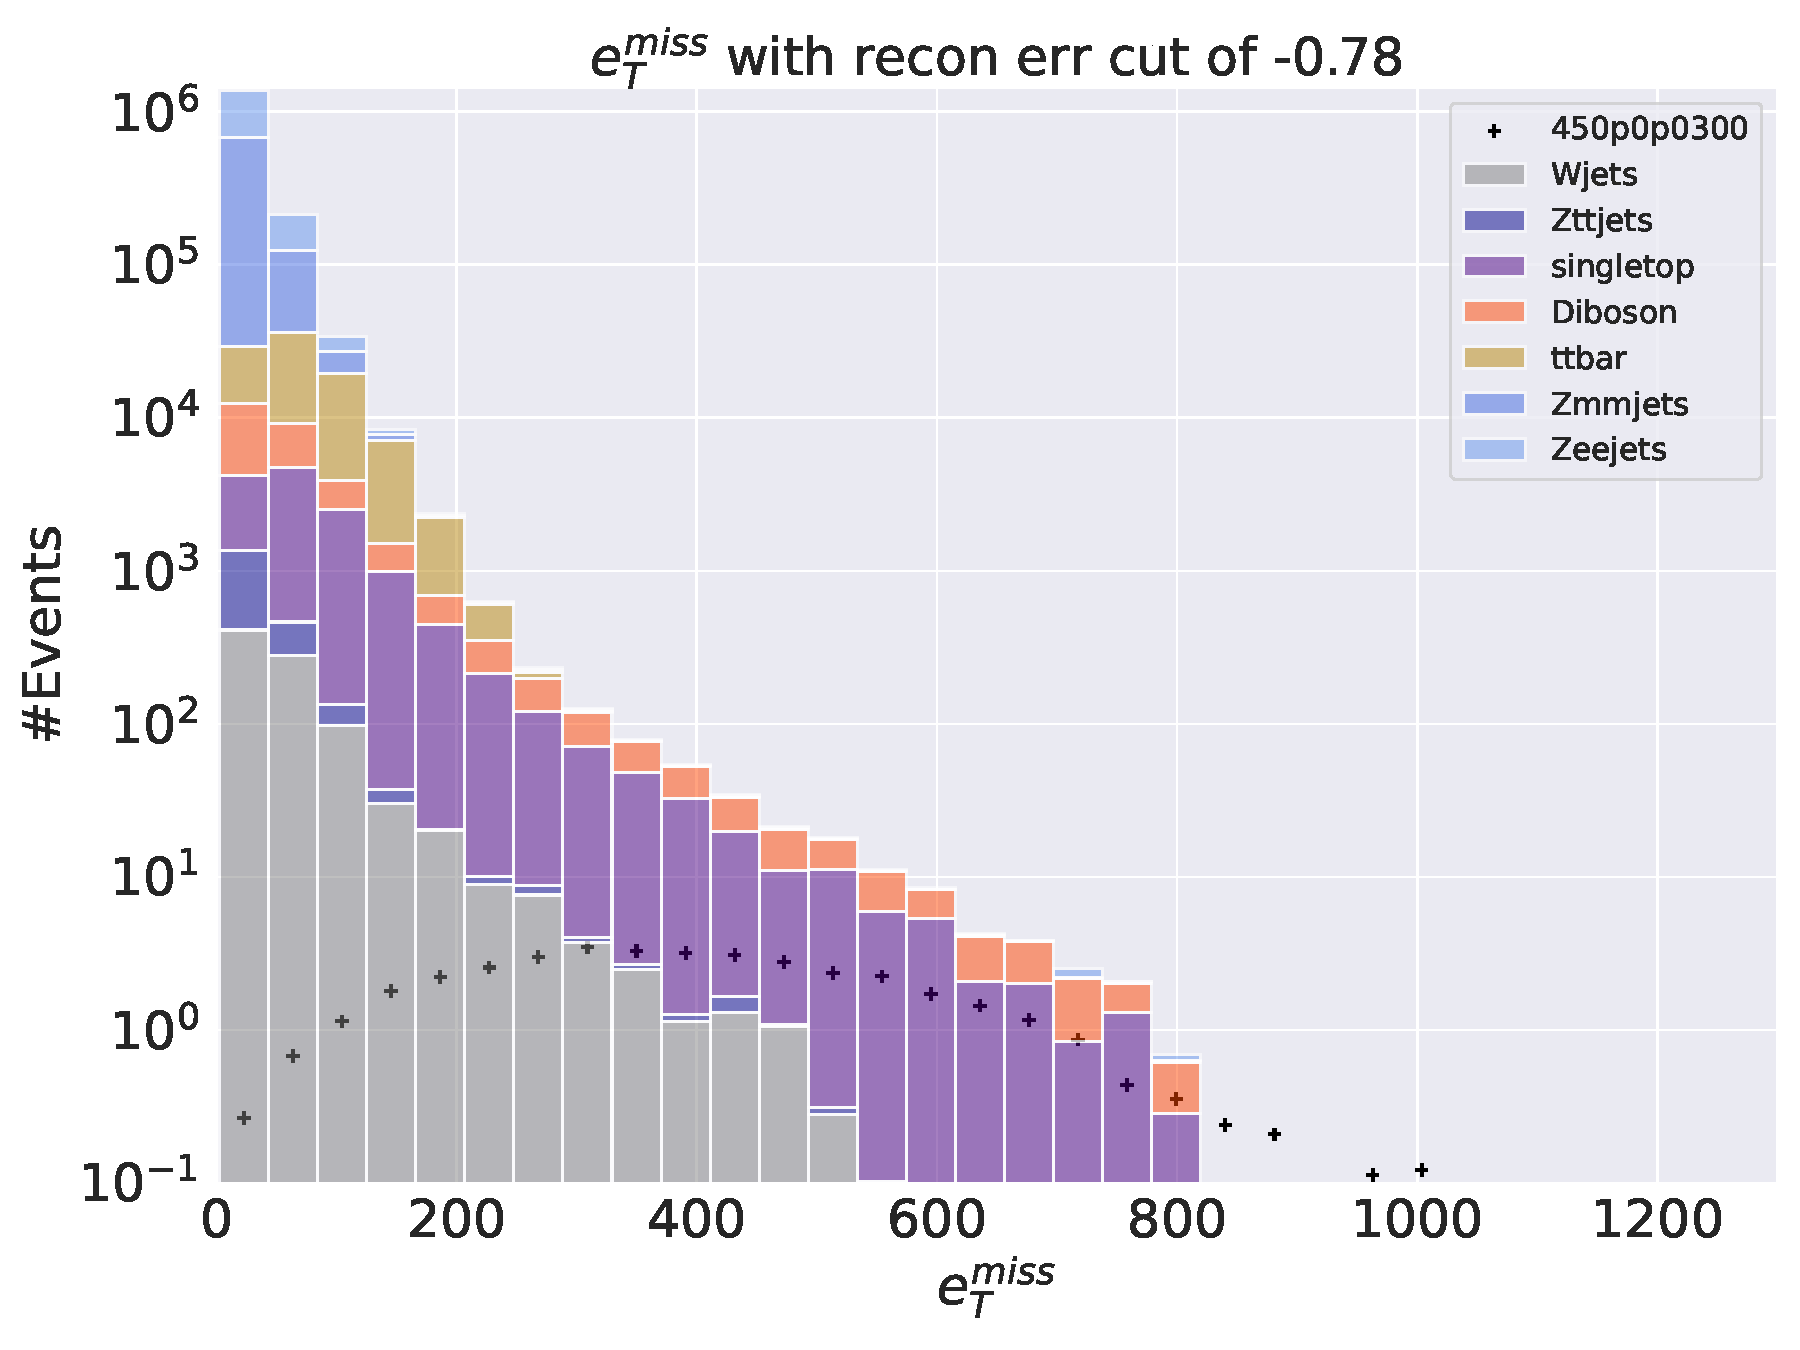
\includegraphics[width=\textwidth]{Figures/VAE_testing/big/2lep/b_data_recon_big_rm3_feats_sig_450p0p0300_recon_errcut_-0.78.pdf}
        \caption{ }
        \label{fig:VAE_2lep_big_450_cut_etmiss}
    \end{subfigure}
    \hfill
    \begin{subfigure}{.45\textwidth}
        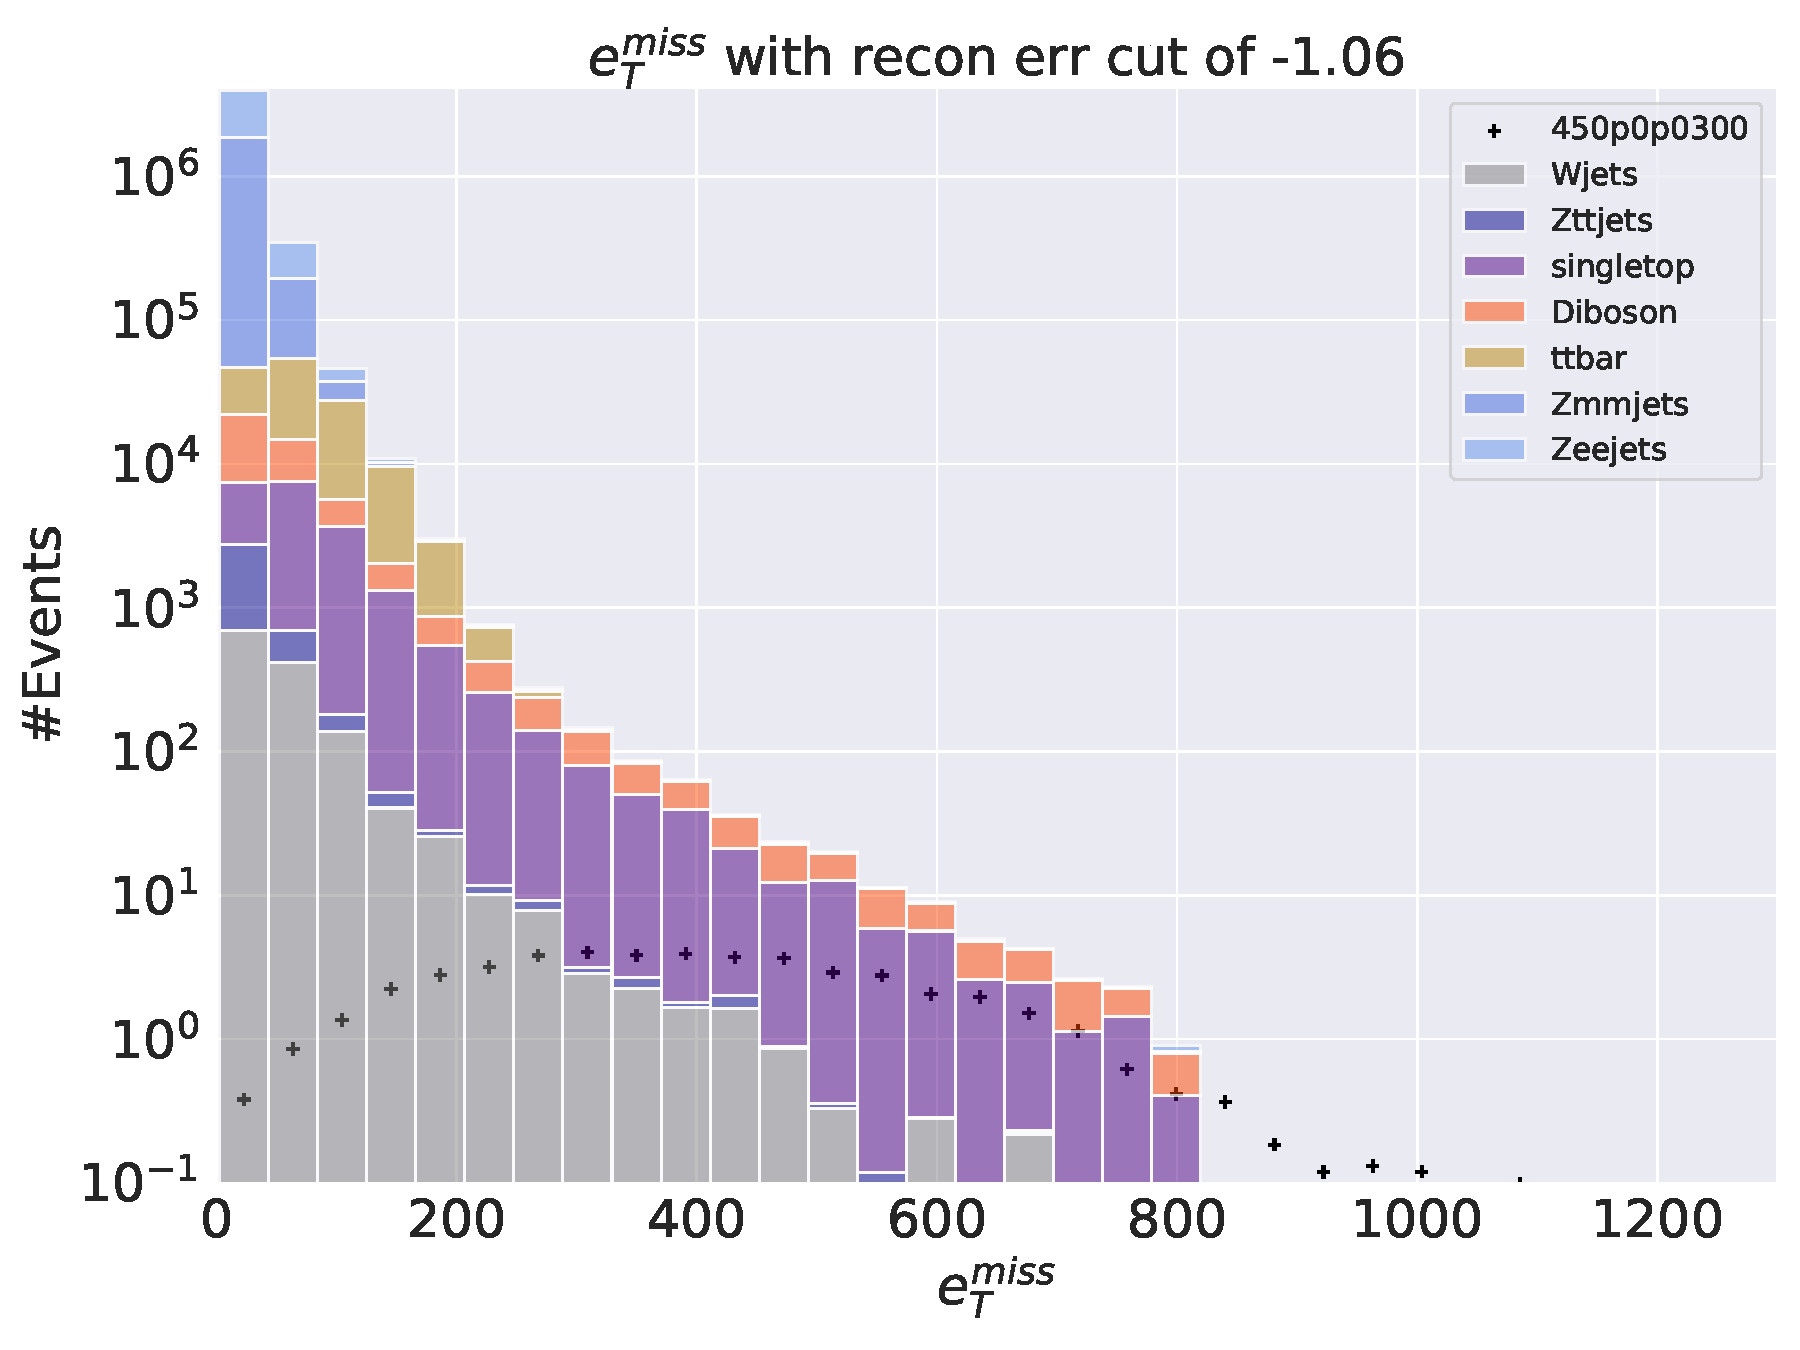
\includegraphics[width=\textwidth]{Figures/VAE_testing/small/2lep/b_data_recon_big_rm3_feats_sig_450p0p0300_recon_errcut_-1.06.pdf}
        \caption{}
        \label{fig:VAE_2lep_small_450_cut_etmiss}
    \end{subfigure}
    \hfill
    \begin{subfigure}{.45\textwidth}
        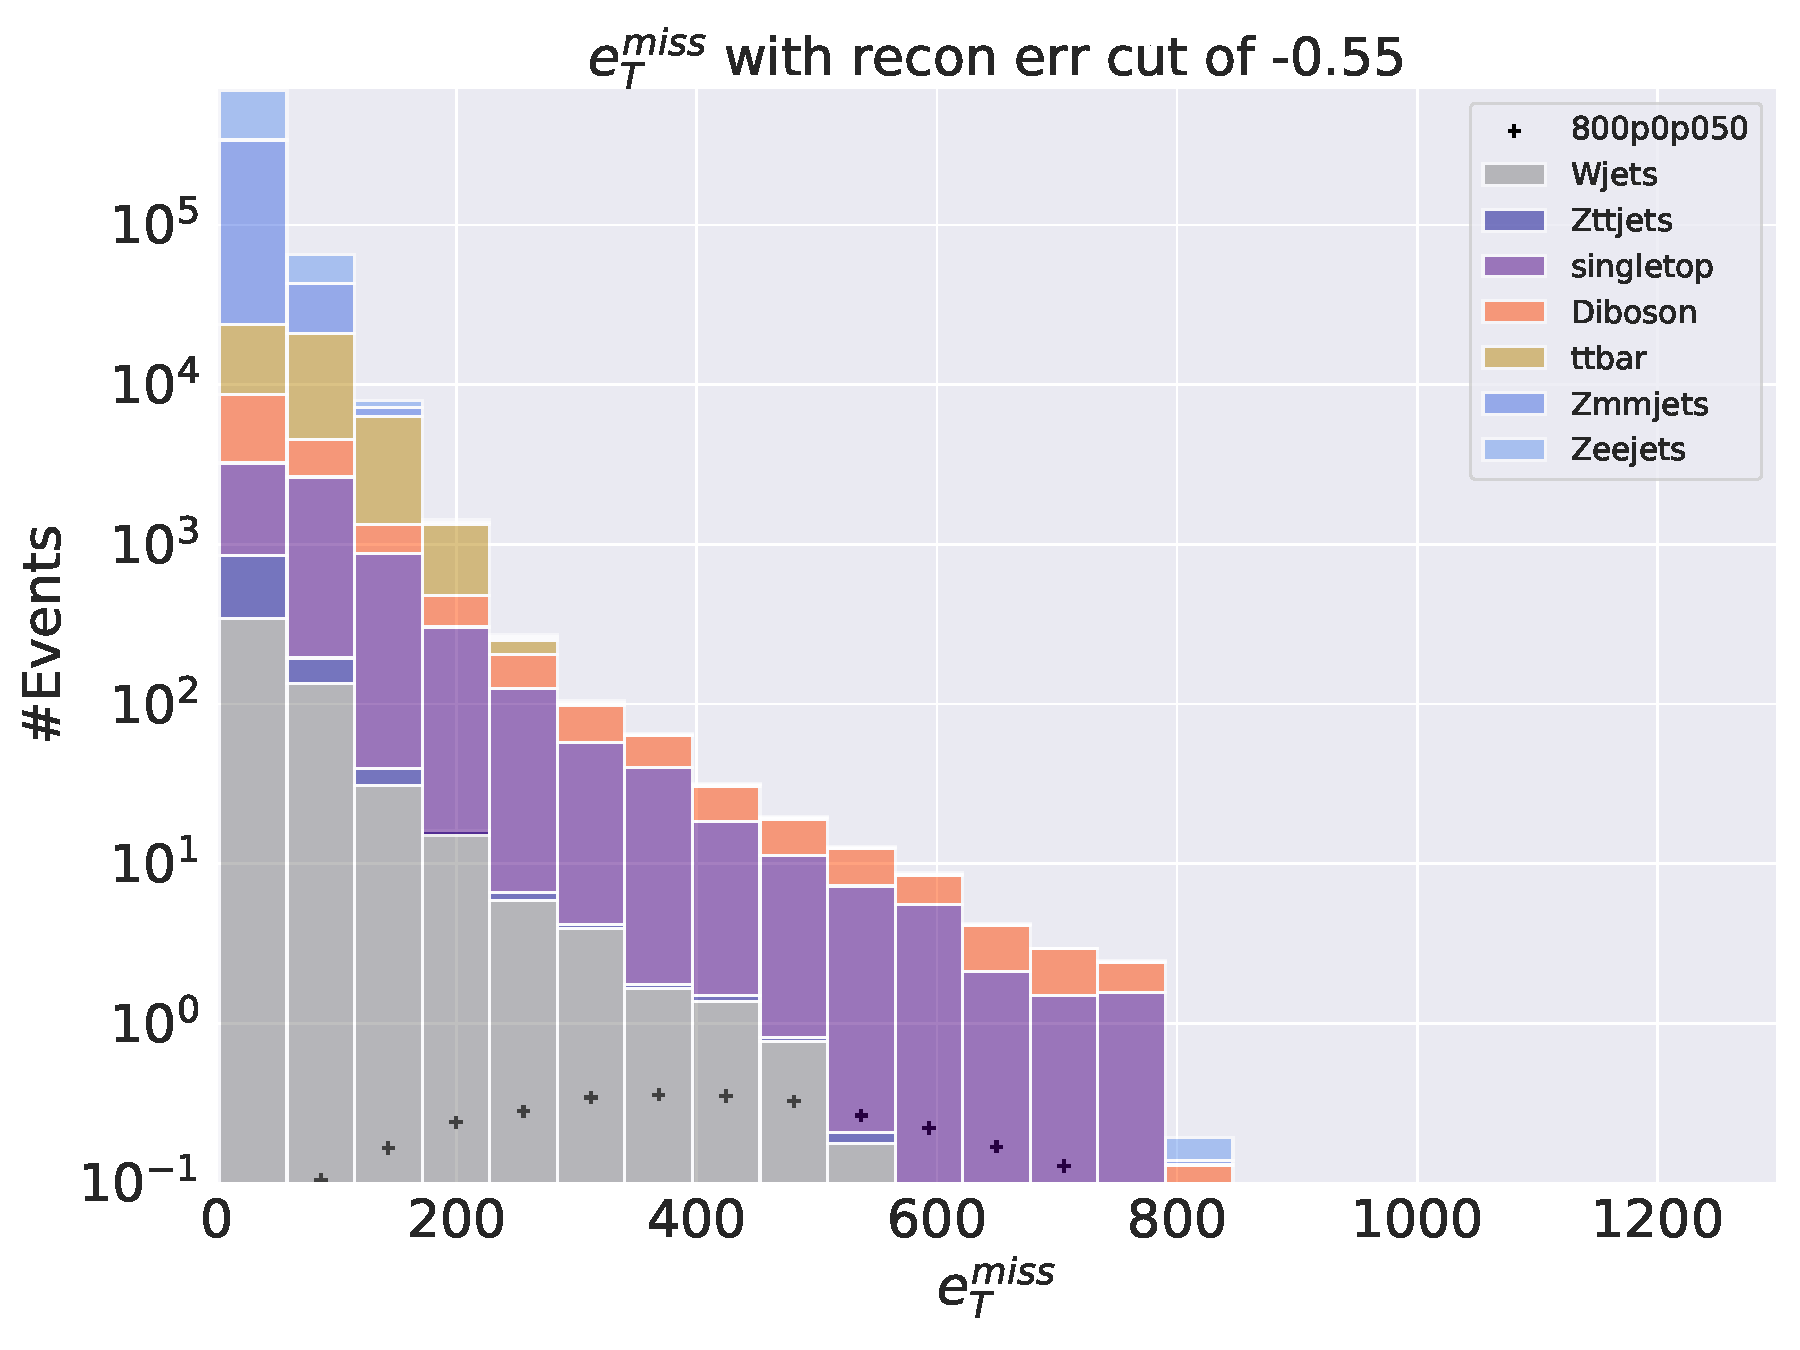
\includegraphics[width=\textwidth]{Figures/VAE_testing/big/2lep/b_data_recon_big_rm3_feats_sig_800p0p050_recon_errcut_-0.55.pdf}
        \caption{}
        \label{fig:VAE_2lep_big_800_cut_etmiss}
    \end{subfigure}
    \hfill   
    \begin{subfigure}{.45\textwidth}
        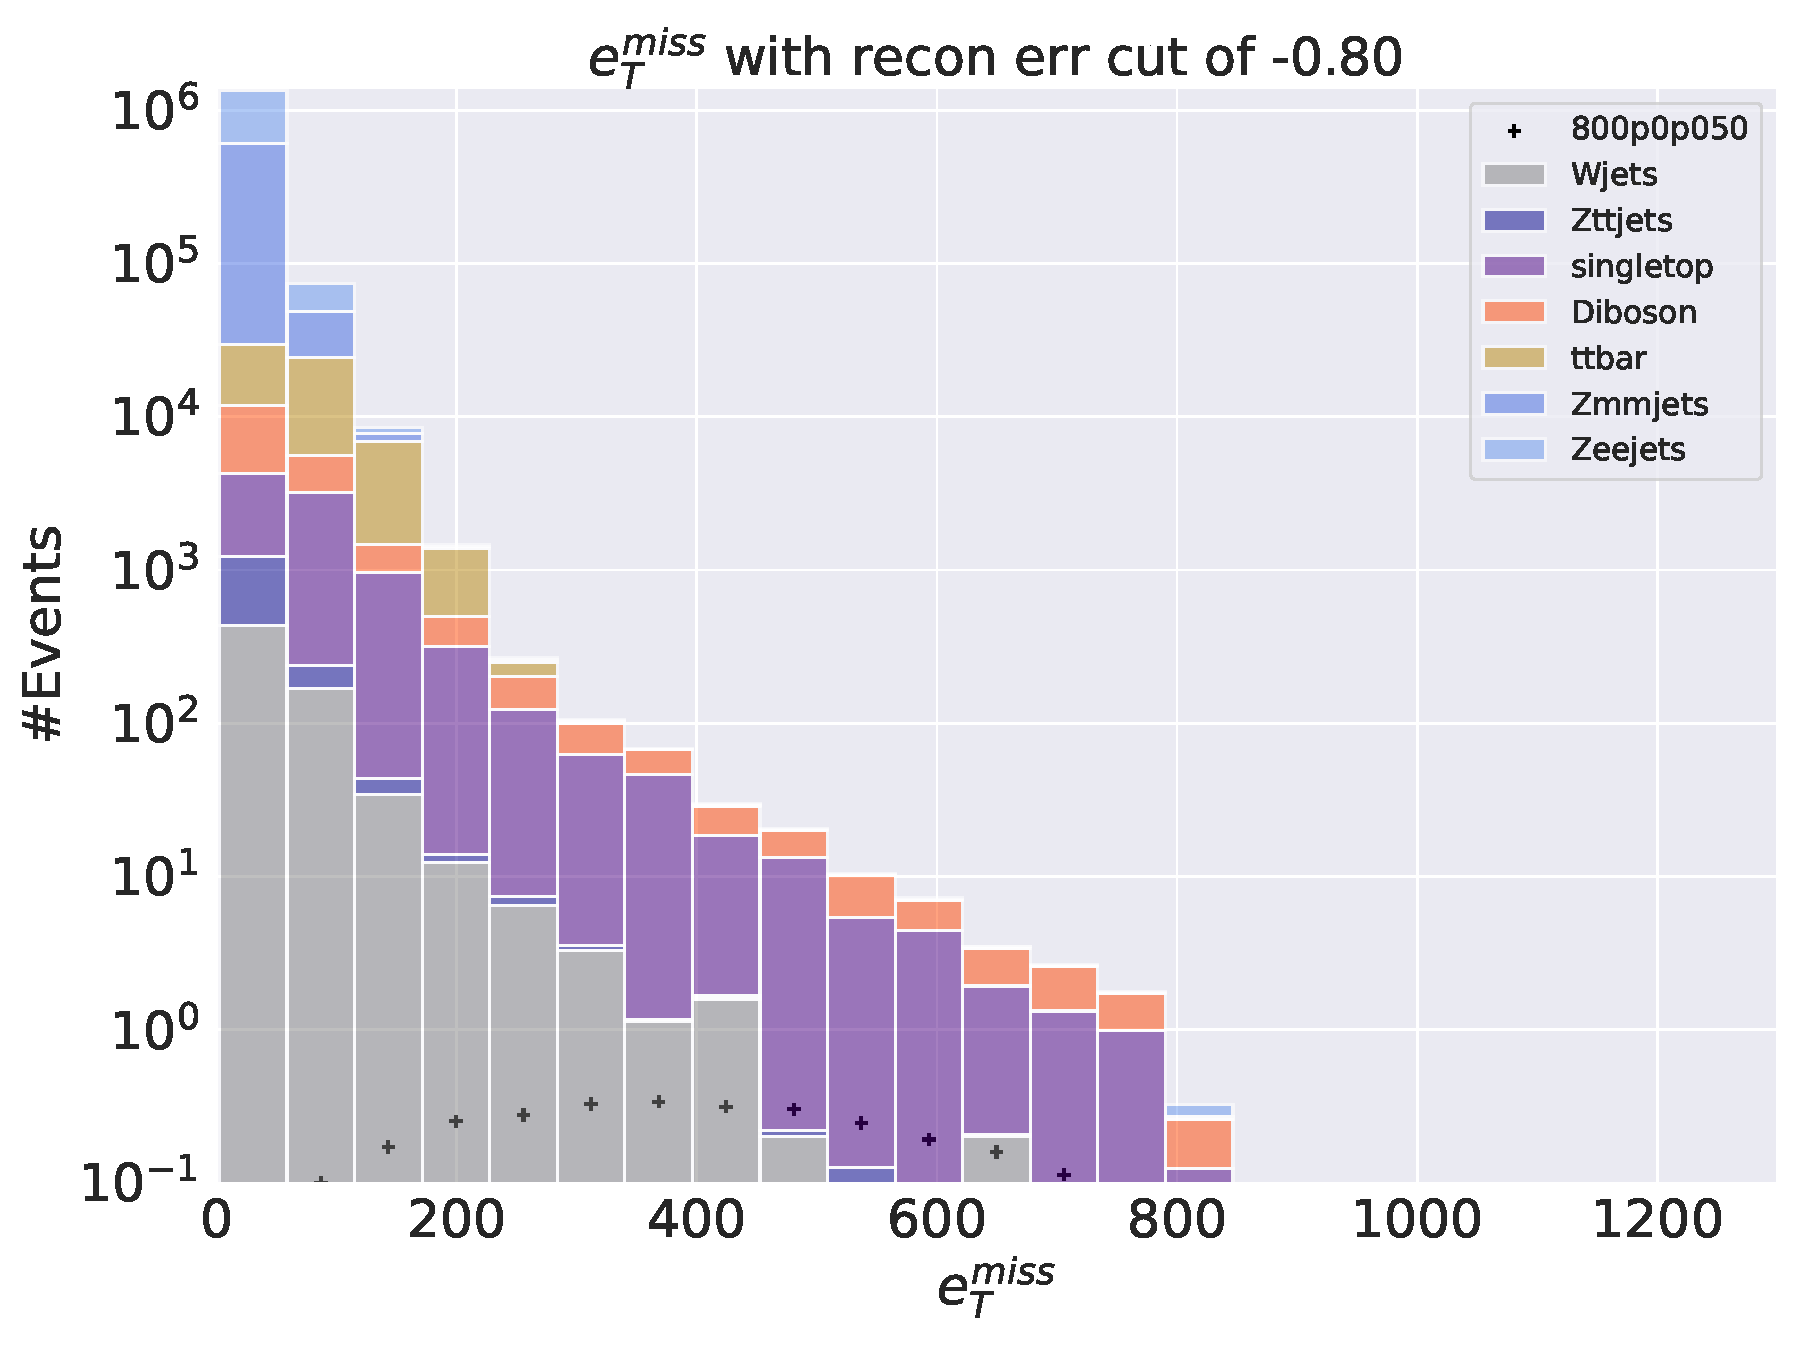
\includegraphics[width=\textwidth]{Figures/VAE_testing/small/2lep/b_data_recon_big_rm3_feats_sig_800p0p050_recon_errcut_-0.80.pdf}
        \caption{}
        \label{fig:VAE_2lep_small_800_cut_etmiss}
    \end{subfigure}
    \hfill      
    \caption[$e_T^{miss}$ best cuts for regular autoencoder]{$e_T^{miss}$ distribution for small (left) and large (right) autoencoder.
    Each figure used the best cut of three possibilities, the remainding results are in the appendix. By best, it is meant that the cut
    gave the best significance. Figures \ref{fig:VAE_2lep_big_450_cut_etmiss} and \ref{fig:VAE_2lep_small_450_cut_etmiss} shows the SUSY 450 and 300 mass signal, 
    and figures \ref{fig:VAE_2lep_big_800_cut_etmiss} and \ref{fig:VAE_2lep_small_800_cut_etmiss} shows the SUSY 800 and 50 mass signal.}
    \label{fig:VAE_2lep_recon_err_both_sig_cut_etmiss}
\end{figure}



WRITE ABOUT THE CUTS DONE IN THE RECONSTRUCTION ERROR DISTRIBUTION



\begin{table}[H]
    \centering
    \caption[Significance table variational autoencoder]{Significance table for the variational autoencoder models. For each signal for both the small and 
    large regular autoencoder, the significance is calculated with equation small (left column) and equation large (right column). The 
    reconstruction error cuts used where $[-0.78, -0.58, -0.39]$ for the SUSY $450p300$ signal and $[-0.74, -0.55, -0.37]$ for the SUSY 
    $800p50$ signal for the large autoencoder. The reconstruction error cuts used for the small autoencoder where $[-1.06, -0.79, -0.53]$ 
    for the SUSY $450p300$ signal and $[-1.06, -0.79, -0.53]$ for the SUSY $800p50$ signal. }
    \label{tab:VAE_2lep_significance}
    \begin{tabular}{|llllllll|}
    \hline
    \multicolumn{8}{|c|}{Regular Autoencoder}                                                                                                                                    \\ \hline
    \multicolumn{4}{|c|}{Small}                                                                    & \multicolumn{4}{c|}{Large}                                                  \\ \hline
    \multicolumn{2}{|l|}{450p300}                  & \multicolumn{2}{l|}{800p50}                   & \multicolumn{2}{l|}{450p300}                  & \multicolumn{2}{l|}{800p50} \\ \hline
    \multicolumn{8}{|c|}{Pre reconstruction error cut significance}                                                                                                                           \\ \hline
    \multicolumn{1}{|l|}{0.017} & \multicolumn{1}{l|}{0.017} & \multicolumn{1}{l|}{0.001} & \multicolumn{1}{l|}{0.001} & \multicolumn{1}{l|}{0.017} & \multicolumn{1}{l|}{0.017} & \multicolumn{1}{l|}{0.001}  & \multicolumn{1}{l|}{0.001} \\ \hline
    \multicolumn{8}{|c|}{Post reconstruction error  cut significance}                                                                                                                         \\ \hline
    \multicolumn{1}{|l|}{0.023} & \multicolumn{1}{l|}{0.023} & \multicolumn{1}{l|}{0.002} & \multicolumn{1}{l|}{0.002} & \multicolumn{1}{l|}{0.030} & \multicolumn{1}{l|}{0.030} & \multicolumn{1}{l|}{0.004}   & \multicolumn{1}{l|}{0.004}  \\ \hline
    \multicolumn{1}{|l|}{0.021} & \multicolumn{1}{l|}{0.022} & \multicolumn{1}{l|}{0.003} & \multicolumn{1}{l|}{0.003} & \multicolumn{1}{l|}{0.026} & \multicolumn{1}{l|}{0.026} & \multicolumn{1}{l|}{0.004}   & \multicolumn{1}{l|}{0.004}  \\ \hline
    \multicolumn{1}{|l|}{0.016} & \multicolumn{1}{l|}{0.016} & \multicolumn{1}{l|}{0.002} & \multicolumn{1}{l|}{0.002} & \multicolumn{1}{l|}{0.018} & \multicolumn{1}{l|}{0.018} & \multicolumn{1}{l|}{0.003}   & \multicolumn{1}{l|}{0.003} \\ \hline
    \end{tabular}
\end{table}

